\newpage
\chapter{Hardware implementation}
\label{sec:implementation}
The following chapter describes the implementation of the ACAD anomaly detector on a Zynq Z-7030 or Z-7035 device, used for the NTNU Smallsat project. \\
 
 A prototype version should be tested on the ZedBoard Zynq Evaluation and Development Kit, having a Z-7020 device.


\section{Top level architecture}

The top level architecture of the ACAD Anomaly detector is shown in Figure \ref{fig:top_level_ACAD}. It consists of five blocks; \textbf{FSM ACAD}, \textbf{Shiftregister\_four\_bands}, \textbf{ACAD correlation module}, \textbf{ACAD inverse module Gauss Jordan} and \textbf{dACAD module}.

\begin{figure}[H]
\refstepcounter{figure}
\begin{tabular}{c|c}

   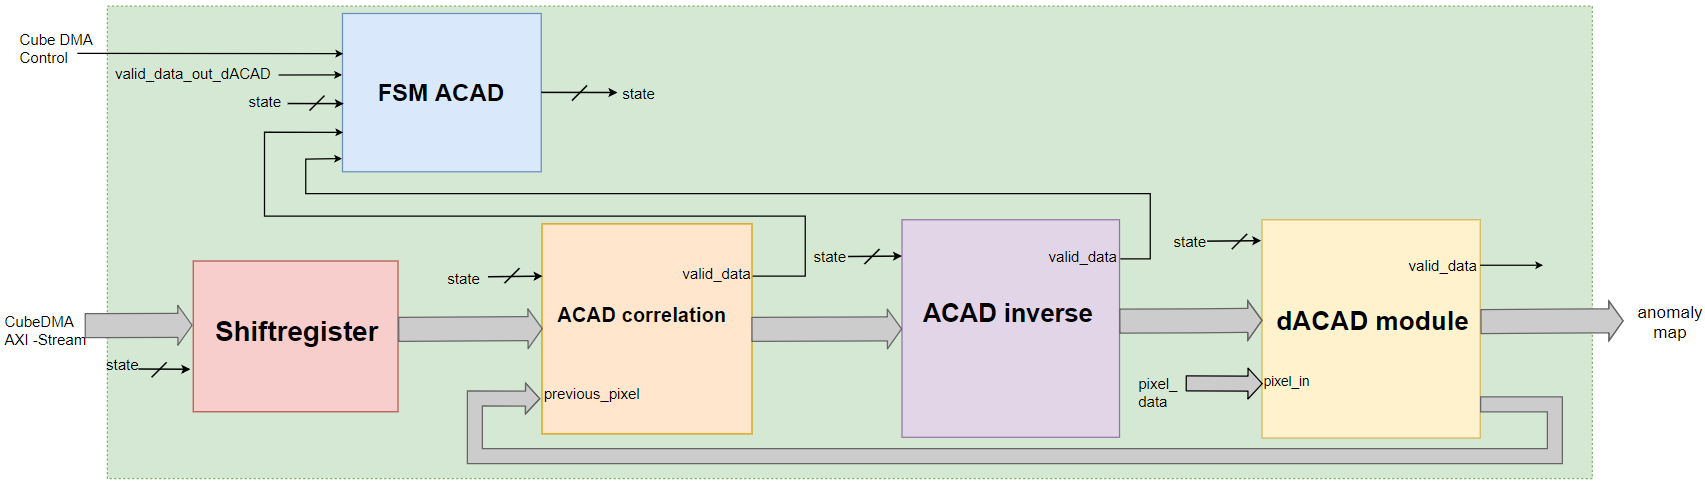
\includegraphics[scale=0.6, angle=90, origin=c]{images/acad_top_level.PNG}
   \rotatebox[origin=c]{90}{ Figure~\thefigure: Top level architecture of the ACAD anomaly detector.}
  %\caption{ \textbf{ROTATE}FSM controlling the architecture shown in Figure  } 
  \end{tabular}
  \label{fig:top_level_ACAD}
\end{figure}

\section{Memory considerations}
\label{sec:memory_management}
    As the ACAD anomaly detector is to be implemented on a Zynq Z-7030 or Z-7035 device, care must be taken when designing, with respect to logic and memory usage. As the hyperspectral image data inputted to the AD might have $P\_BANDS$=100, with 16-bit image data per spectral band, memory usage is an important consideration.   

\subsection{Correlation matrix}
\label{sec:mem_management_correlation_matrix}
Storing and updating the causal correlation matrix sum as shown in equation \ref{eq:caus_corr} requires a lot of memory resources. This update needs to be done for each pixel in the image, and the memory used for this operation is therefore important in order to make the AD real-time. The size of the correlation matrix will be $p * p$, where $p$ is the number of spectral bands in the image. As mentioned, the number of usable bands $N_{bands}$ is 100. The image pixel data width, $pixel\_data\_width$ is assumed to be 16 bit/band/pixel. As the correlation matrix is the product of $\textbf{x}$ * $\textbf{x}^T$ the resulting correlation pixel width will be 2* $pixel\_data\_width$. Using spectral information from all the bands would require $p * p * 32$= $100$ *$100$ *$32$ bit = $320 kbit$ of memory storage. 
\\

There are three alternatives to storing all this information on the FPGA; storing it in block RAM, distributed RAM/LUTRAM or in registers. The FPGA to be used in the SmallSat's first prototype is the Zynq Z-7030 or the Zynq Z-7035. 
The FPGAs contains the memory resources as shown in figure \ref{fig:zynq_memory_resources}.





\begin{figure}[H]
\centering                                                              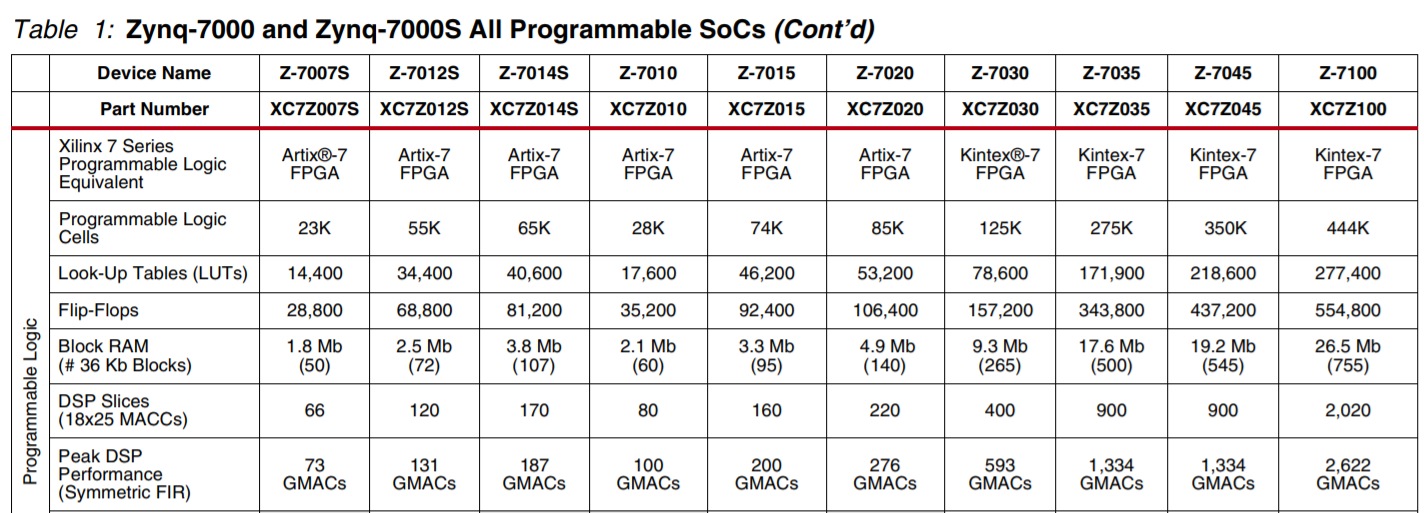
\includegraphics[scale=0.5]{images/zynq_memory_resources.PNG}
  \caption{Zynq memory resources, found in \cite{cite:mem_resources_zynq}.} 
  \label{fig:zynq_memory_resources}.
\end{figure}

\subsubsection{Using registers}
The Zynq Z-7030 and the Zynq Z-7035 have $157,200$ and $343,800$ flip flops each, respectively. Using equation \ref{eq:max_bands}, the maximal number of spectral bands used is 70 and 103. However, this is unrealistic as this leaves no flip flop free for other use in the design. As the AD implemented in this task is a part of a larger processing pipeline (insert picture of pipeline somewhere?) it is not acceptable to use all of the available flip flops. Assuming that it is acceptable to use 15\% of the available flip flops, the number of spectral bands that can be used is 27 and 40 for the Zynq Z-7030 and the Zynq Z-7035 respectively. This dimensional reduction can be done through pre-prossesing of data by for example Principal Component Analysis(PCA). (insert result showing AD doing better with PCA in front?). 
The benefit of the use of registers is the speed and the ability of instantaneous update. %This will lead to the AD becoming closer to real-time than if distributed RAM or BRAM is used.

\begin{equation}
    max\_bands= \sqrt{\frac{number\_of\_registers}{2*pixel\_data\_width}}
    \label{eq:max_bands}
\end{equation}

\subsubsection{Using BRAM}
The Z-7030 and the Z-7035 contains 265 and 500 $36$kbit BRAM - blocks respectively. In  order to store the largest correlation matrix of $320 kbit$ a minimum of 9 BRAM blocks are needed. Each 36 kbit BRAM block consists of two 18 kbit BRAM blocks. In true dual port(TDP) mode \cite{cite:ug953}, it is possible to do two writes and two reads per BRAM per clock cycle, with each write and read being maximum 36 bits. BRAMs in TDP mode have only one address input, the same address for reads and writes. This makes it hard to use for the correlation module, as the ACAD correlation needs to read previously stored data from the BRAM before writing to the same address. Therefore, it is necessary to have a separate read and write address. By inferring two separate Simple Dual Port(SDP) 18kbit BRAMs, by the code shown in Listing \ref{lst:inferr_bram}, it is possible to get two writes and two reads per cycle, with separate read and write addresses. Two SDPs are stored within one 36kbit BRAM block. This is shown in Figure \ref{fig:BRAM_hierarchy}.

\lstinputlisting[caption={Code for inferring a SDP 18 kbit BRAM.},label={lst:inferr_bram},style=customc]{code/bram_espen_sdp.vhd}


\begin{figure}[H]
\centering

   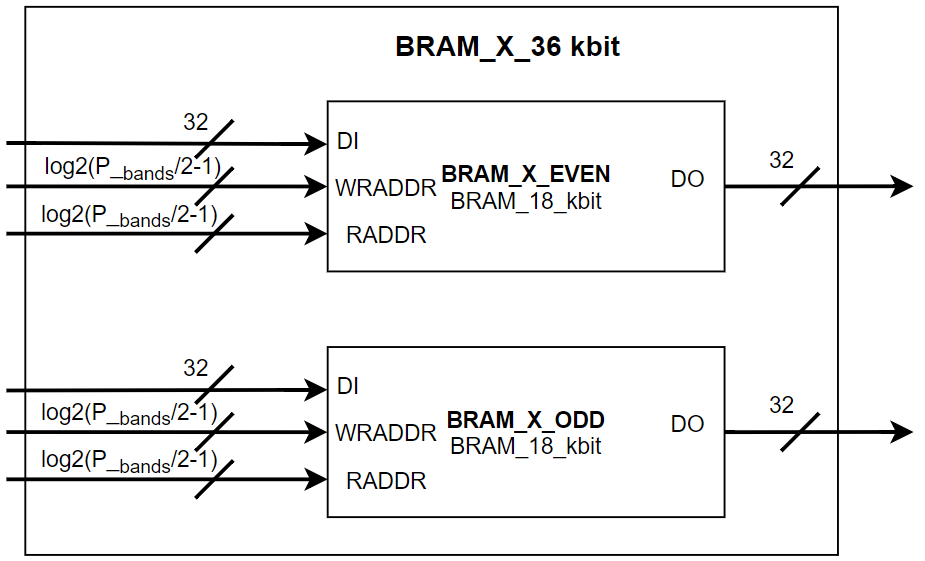
\includegraphics[scale=0.5]{images/BRAM_two_18_kbit.PNG}
  \caption{BRAM hierarchy for correlation module, showing two 18kbit BRAM blocks, contained within one 36kbit BRAM block. } 
  \label{fig:BRAM_hierarchy}
\end{figure}

\\


Equation \ref{eq:clk_cycles_corr_update_BRAM} shows the calculation of number of clock cycles needed to update the correlation matrix, $n\_clk\_update\_corr\_BRAM$. This is done for each pixel in the image. $n\_BRAM$ is the number of 36 kbit BRAMs used to store the correlation matrix. The total time spent updating the correlation matrix for the entire image is given by equation \ref{eq:clk_cycles_corr_image}. Updating a correlation matrix wih $p$ = 100, using 9 BRAMs in TDP mode would require 556 clk cycles. For the entire image, having $N\_pixels$ the total amount of clock cycles spent updating the correlation matrix would be 349648384. At a target clock frequency of 100 MHz this would require $3.49648$ seconds, which is not to be considered real time.   

\begin{equation}
    n\_clk\_update\_corr\_BRAM = \frac{p * p }{2 * n\_BRAM}
    \label{eq:clk_cycles_corr_update_BRAM}
\end{equation}

\begin{equation}
    clk\_corr\_image\_BRAM = N\_pixels *number\_of\_lines * n\_clk\_update\_corr\_BRAM
    \label{eq:clk_cycles_corr_image}
\end{equation}


Figure \ref{fig:update_time_correlation_BRAM} shows the total time spent updating the correlation matrix for a image of 1088 pixel rows with 578 effective pixels per row, with a target clock frequency of 100 MHz. The BRAMs are assumed written to in parallel.  

\begin{figure}[H]
\centering
\hbox{\hspace*{-2cm}                                                           

   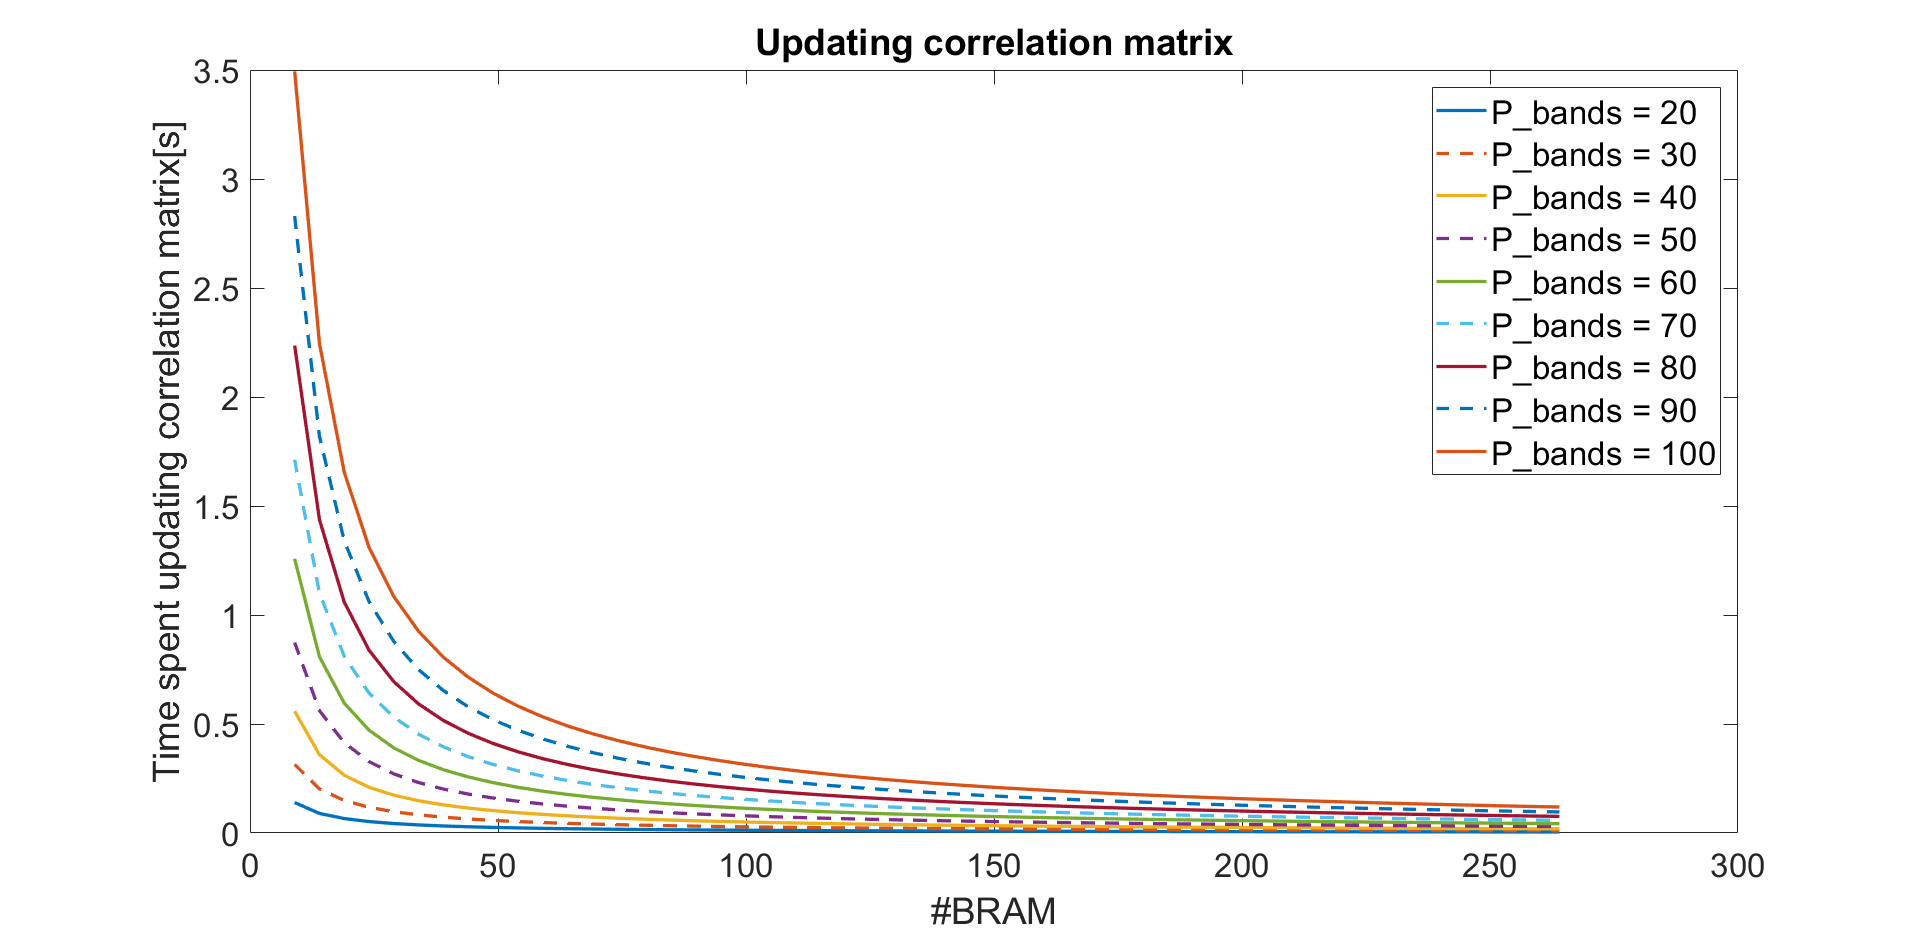
\includegraphics[scale=0.3]{images/time_spent_updating_correlation_matrix.png}}
  \caption{Estimated time spent updating correlation matrix for an image of 1088 pixel rows with 578 effective pixel per row, with a target clock frequency of 100 MHz, plotted as a function of number of 36 kbit BRAMs used to store and update the correlation matrix. Plotted for spectral bands in the range of P=20 to P=100. } 
  \label{fig:update_time_correlation_BRAM}
\end{figure}

\section{Shiftregister\_four\_bands}



\section{ACAD correlation}
\label{sec:correlation_hw}
The \textbf{ACAD correlation module}, as shown in Figure \ref{fig:top_level_ACAD}, computes the ACAD correlation matrix $\Tilde{\textbf{R}}_{k x k}(\textbf{x}).
\\

As the SmallSat project is in the early phases, the value of $p$ for the data inputted to the AD from preprocessing steps are insecure. Another insecurity is the performance of the ACAD AD using PCA pre-processing, i.e. reducing the number of spectral bands in the AD. In addition, the ACAD AD requires storing of the inverse matrix, and the sum of anomaly detected. This is shown in figure X ( insert a figure showing the equation and what needs to be stored where). It is therefore not desirable to store the entire correlation matrix in flip flops, as there will be a need for storing other matrices, either in BRAM or DRAM, thereby inserting a bottleneck in the pipeline relative to the flip flop-updating step. Using BRAMs it is also possible to make a scalable solution for both small and large $p$. 
\\


As shown in Figure \ref{fig:update_time_correlation_BRAM} the time spent updating the correlation matrix can be reduced by increasing number of 36kbit BRAMs used to store the correlation matrix. By setting the  number of 36kbit BRAMs used to store the correlation matrix, $N\_BRAMS\_correlation$, equal to $P\_BANDS$ it is possible to store one column of the correlation matrix in each BRAM. This simplifies the control logic while achieving an acceptable trade off between speedup as a function of number of BRAMs used and resources used. Figure \ref{fig:data_flow_cube_dma_to_inverse} shows the data flow from the Cube DMA through the ACAD correlation module, with $N\_BRAM\_correlation$ =$P\_BANDS$. 
\\


\begin{figure}[H]
\centering
   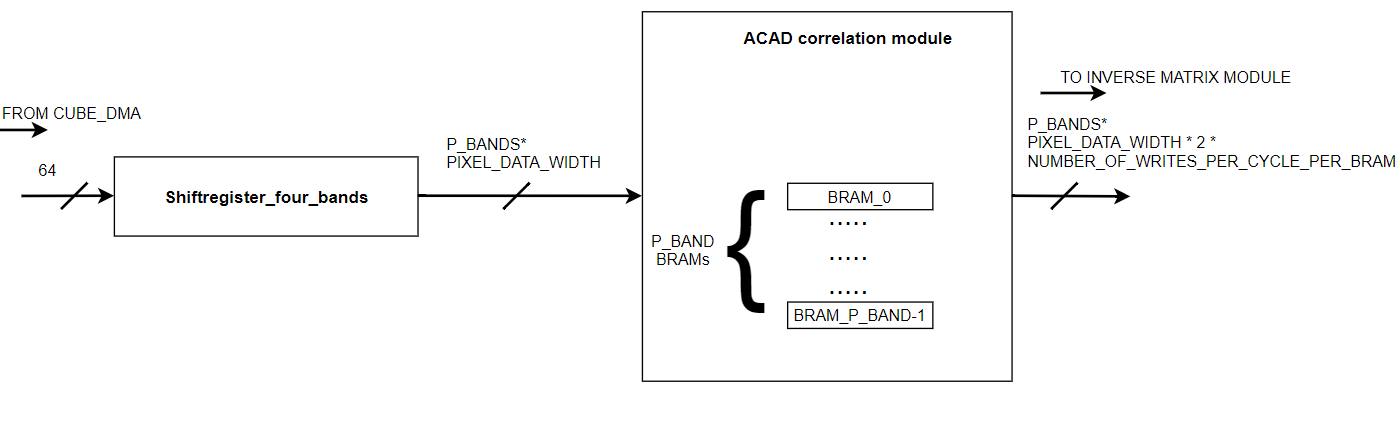
\includegraphics[scale=0.5]{images/data_flow_cube_dma_to_inverse_module.PNG}
  \caption{Data flow from Cube DMA via shiftregister to correlation module. Output on right hand side are input for inverse matrix computation module.  } 
  \label{fig:data_flow_cube_dma_to_inverse}
\end{figure}

Setting $N\_BRAMS\_correlation$ = $P\_BANDS$ allows to write to $P\_BANDS$ number of columns of the correlation matrix at the same time. As it is possible to write two 32 bit elements per cycle for each 36 kbit BRAM block, the total correlation matrix update time per pixel is $\frac{P\_BANDS}{2}$. 


The design is made for an even number of $P\_BANDS$. If odd number of spectral band is used, a band with zero values has to be inserted before inputting to the correlation module.\\

The design is made to be scalable with $P\_BANDS$, and will synthesize $P\_BANDS$ 36 kbit BRAMs and $P\_BANDS * 2$ DSP48E1(used for multiplication). By changing the value of the constant $P\_BANDS$ found in the $common\_types\_and\_functions$ package, the number of correlation sub-modules is changed. These sub-modules are shown in Figure \ref{fig:data_flow_correlation}. 
\begin{figure}[H]
\centering
   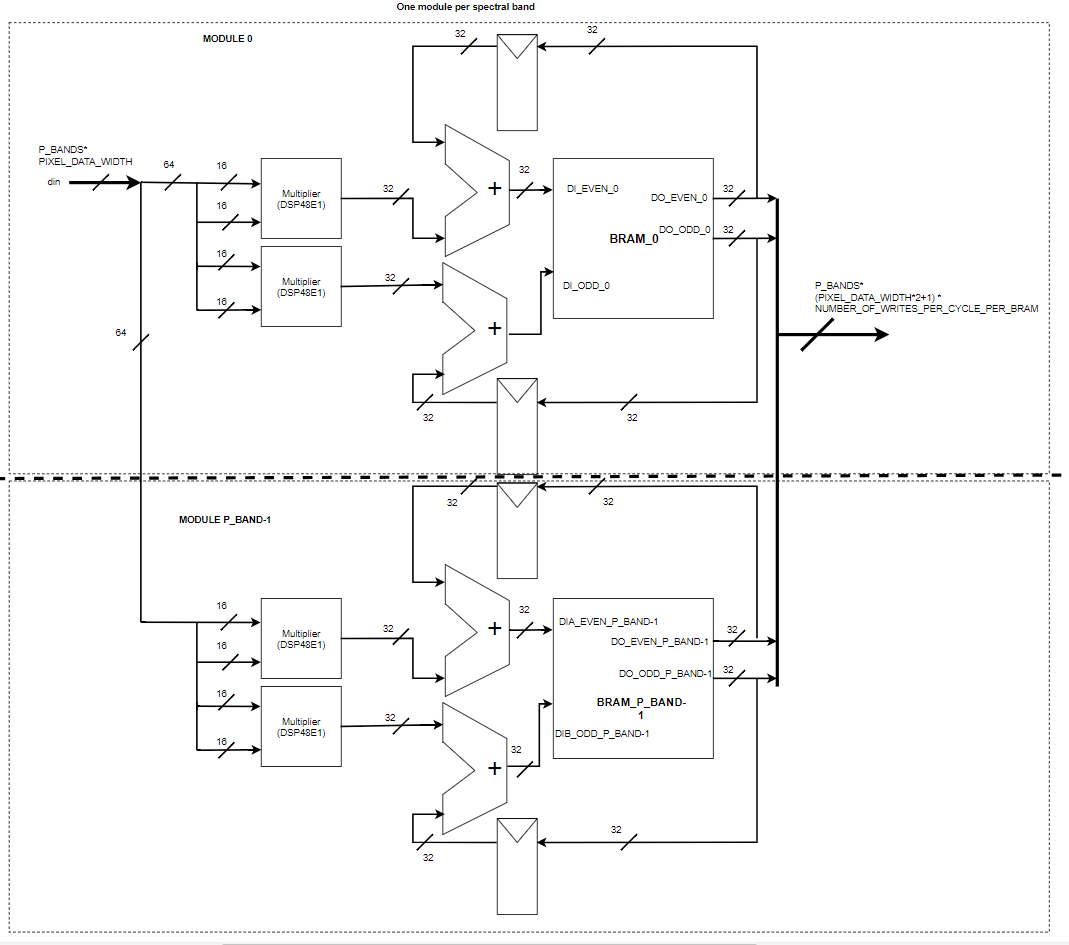
\includegraphics[scale=0.6]{images/correlation_data_path_with_adders.PNG}
  \caption{Data flow within the correlation module. The dotted lines marks one correlation sub-module. $P\_BANDS$ such modules are synthesized in the design. } 
  \label{fig:data_flow_correlation}
\end{figure}

The design was synthesized for $P\_BANDS$=10,20,30,40,50,60,70,80,90,100. Synthesis results show that the design scales as expected with respect to number of BRAM36E1 and DSP48E1 used. Figure \ref{fig:primitves_correlation}  shows the number of synthesized primitives  BRAM36E1 and DSP48E1. Figure \ref{fig:luts_and_regs_corr} shows number of synthesized SLICE REGISTERS and SLICE LUTS as a function of $P\_BANDS$.

\begin{figure}[H]

\hbox{\hspace*{-2cm}                                                           
   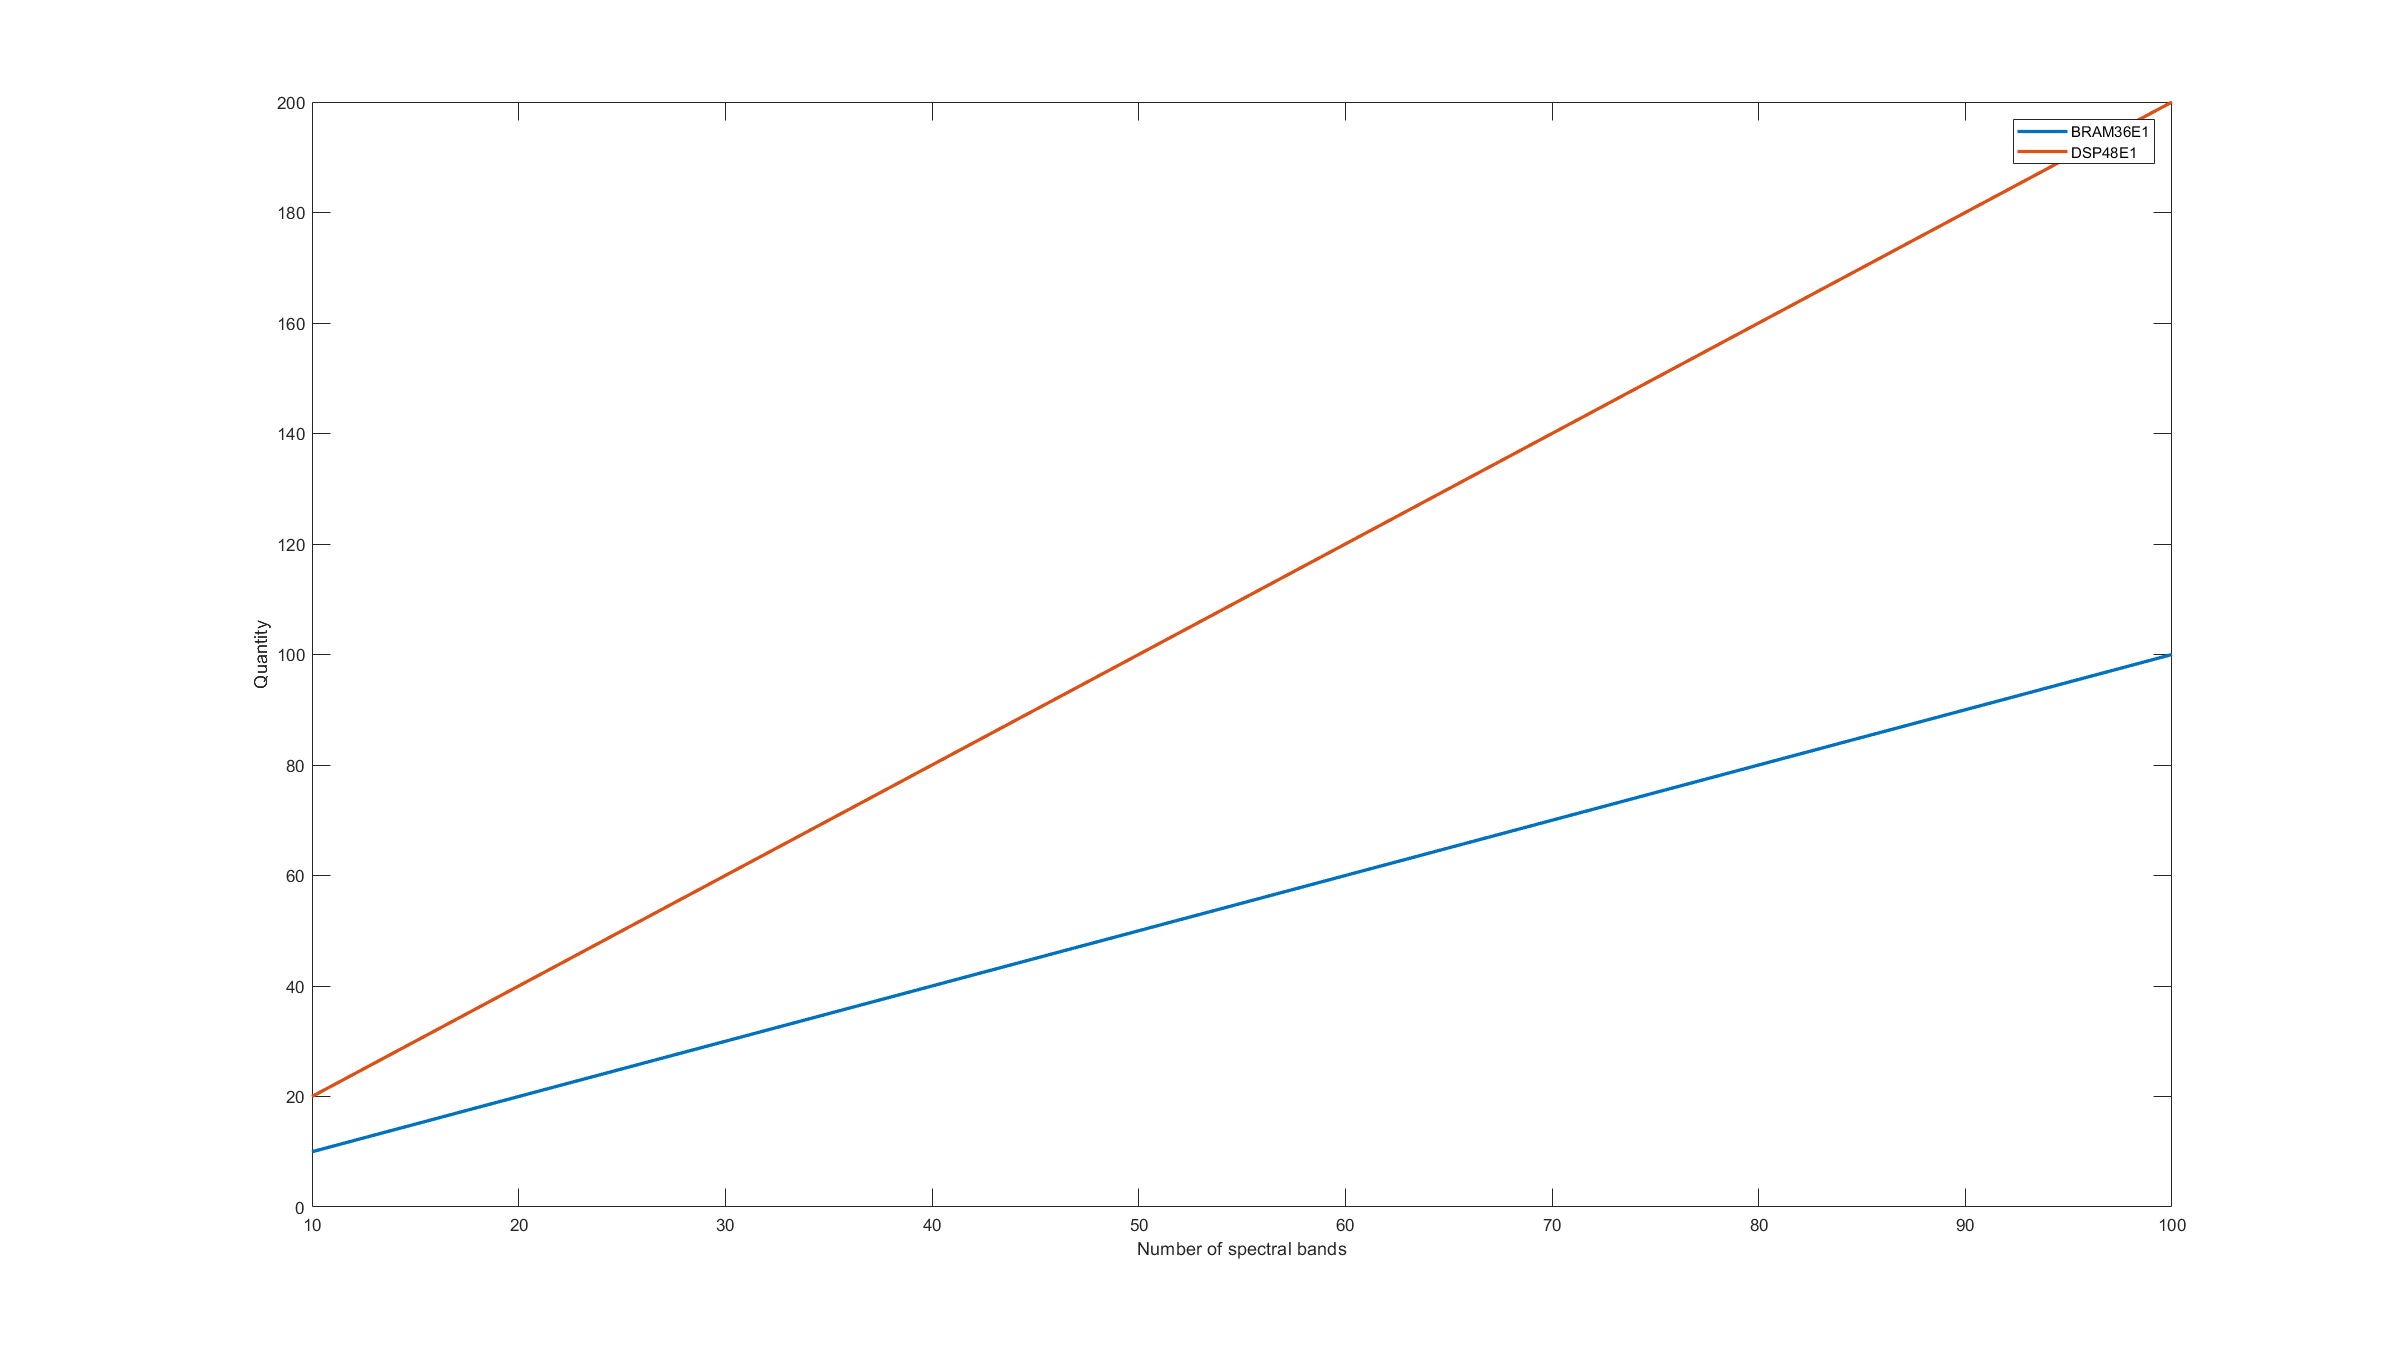
\includegraphics[scale=0.3]{images/number_of_BRAMS_and_DSP48.png}}
  \caption{Number of synthesized BRAM36E1 and DSP48E1 as a function of $P\_BANDS$. Results gathered from synthesis utilization report. } 
  \label{fig:primitves_correlation}
\end{figure}


\begin{figure}[H]

\hbox{\hspace*{-2cm}                                                           
   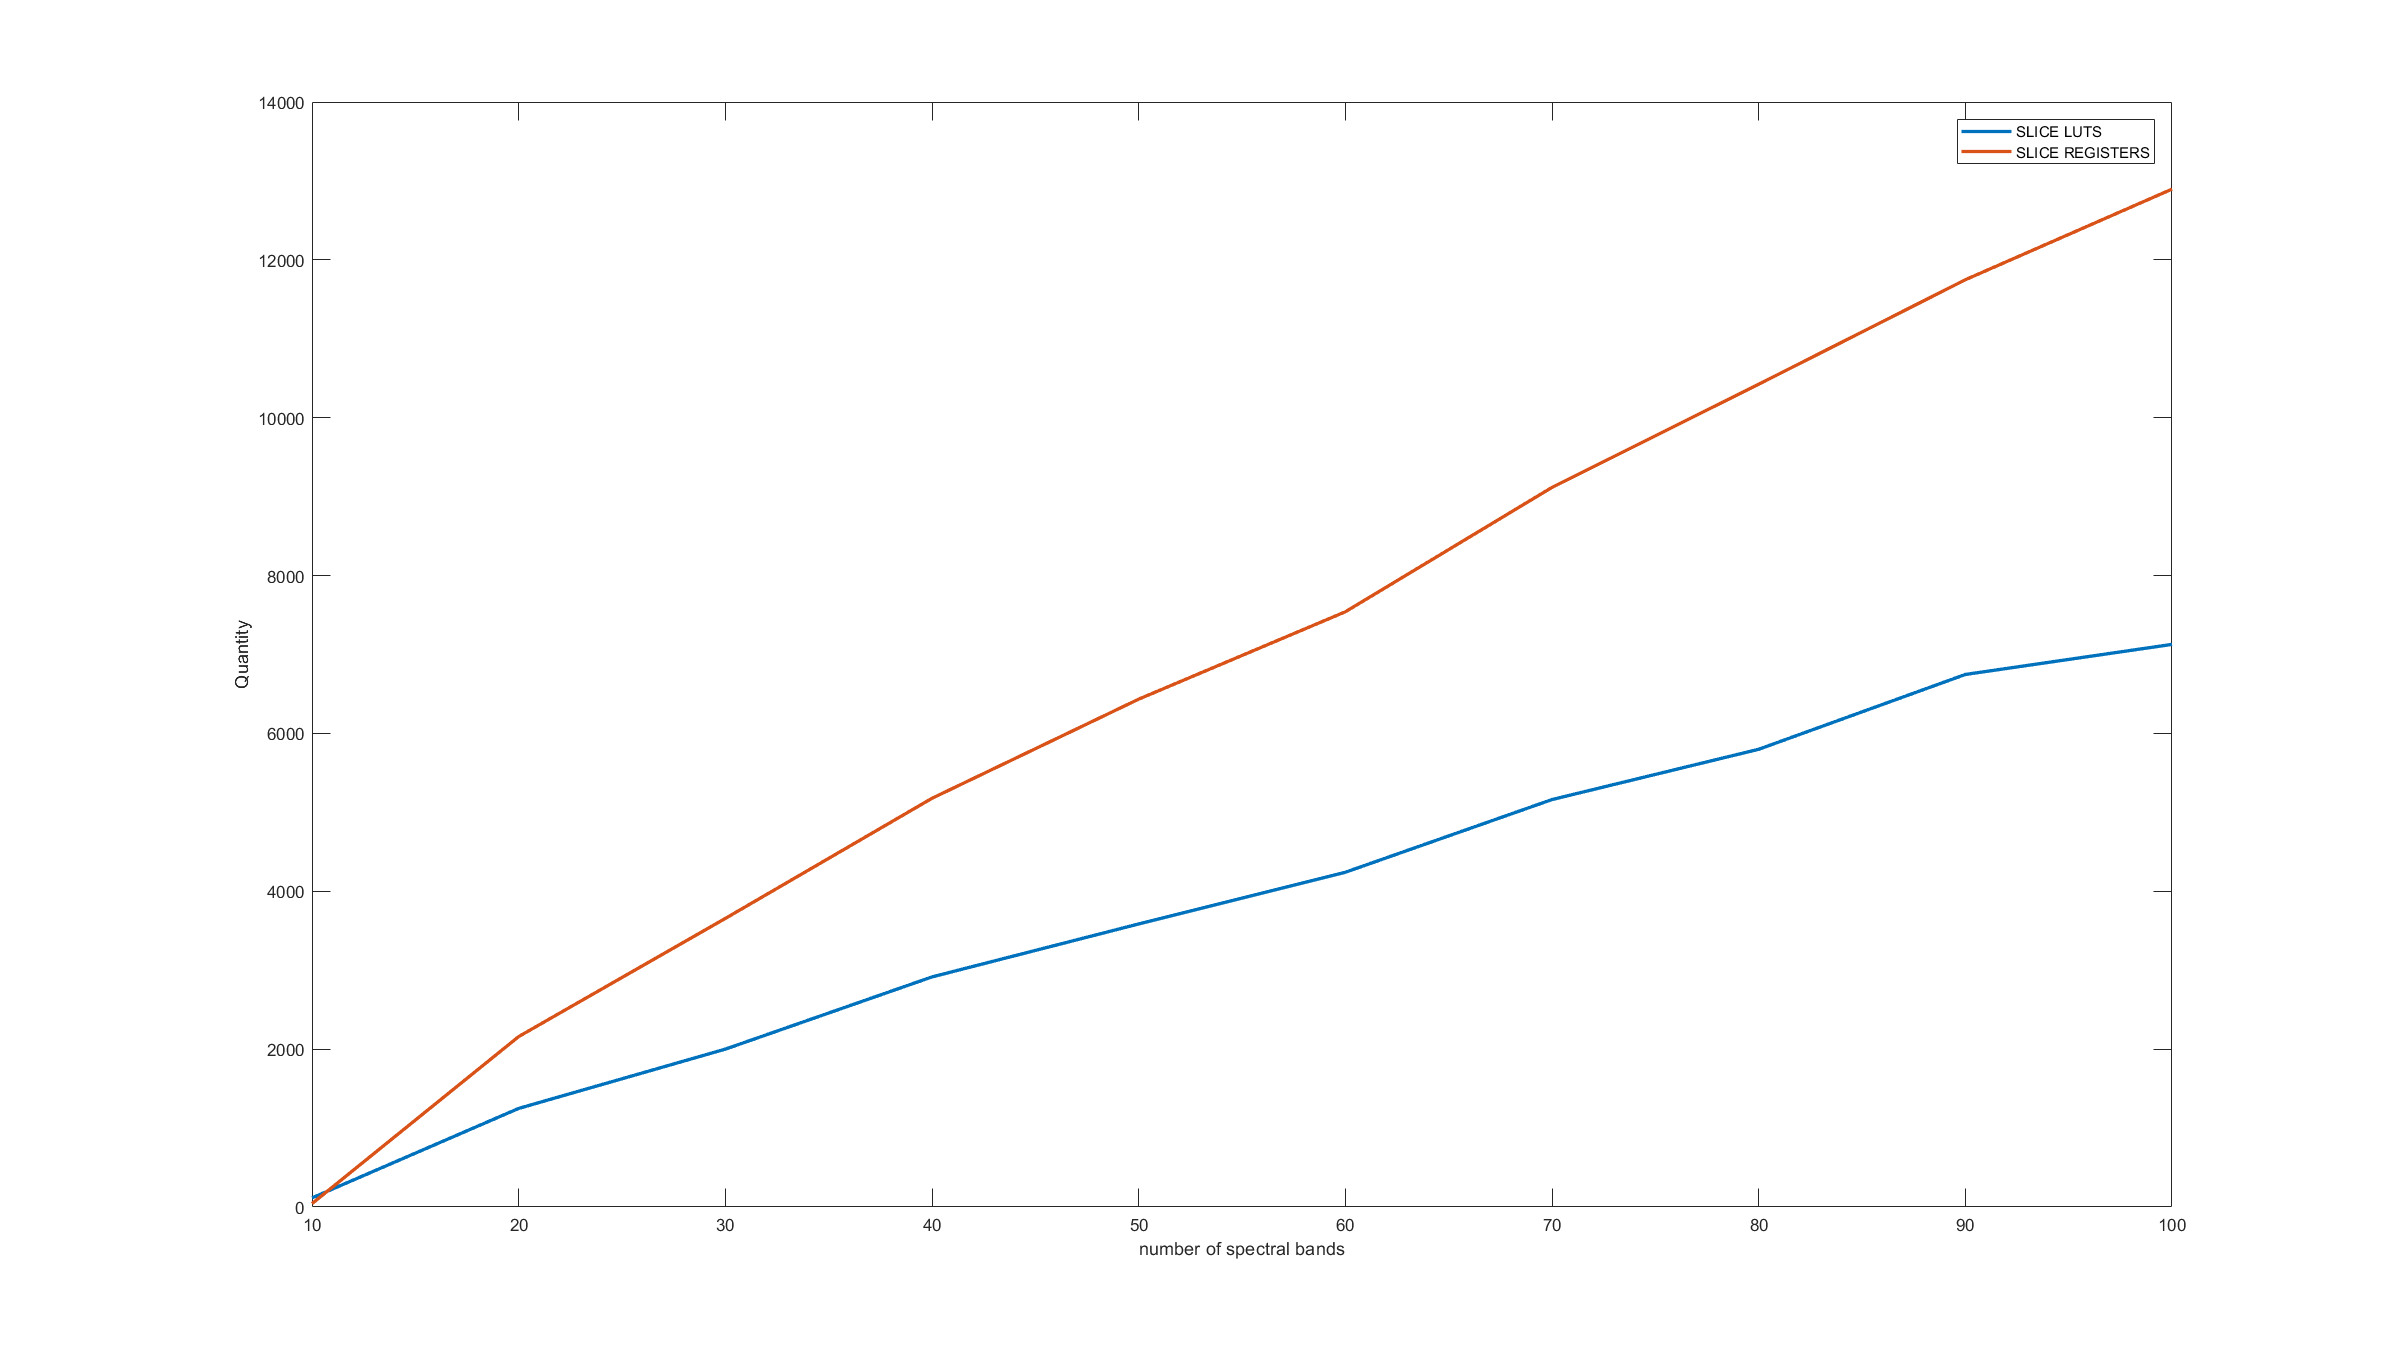
\includegraphics[scale=0.3]{images/correlation_luts_and_registers.png}}
  \caption{Number of synthesized SLICE REGISTERS and SLICE LUTS as a function of $P\_BANDS$. Results gathered from synthesis utilization report. } 
  \label{fig:luts_and_regs_corr}
\end{figure}


Pixel data inputted to the correlation module is inputted as a horizontal vector. For ACAD, the correlation matrix is presented in equation \ref{eq:caus_corr}. The correlation matrix is written to $N\_BRAM\_correlation$ in parallel, where the leftermost column(column zero) of the correlation matrix is written to BRAM\_0, column one to BRAM\_1,.. column P\_BANDS-1 to BRAM\_P\_BANDS-1. For each 36 kbit BRAM, two 18kbit BRAM blocks are accessed, one for even indexes of the column, and one for odd indexes of the column. This is also shown in figure \ref{fig:BRAM_hierarchy}. In Figure \ref{fig:BRAM_matrix} the addressing scheme for each 36kbit BRAM is presented, exemplified by BRAM\_0 and BRAM\_P\_BANDS-1. As shown in the figure, elements of column zero is stored in BRAM\_0, while elements of column P\_BANDS-1 is stored in BRAM\_P\_BANDS-1. Each 36 kbit BRAM consists of two 18 kbit blocks, storing even and odd row-index elements respectively. 

%the write sequence for each 36kbit BRAM is presented, exemplified by BRAM0. Here, the vertical vector element is din[PIXEL\_DATA\_WIDTH-1:0], shown by the blue line. The green lines shows data processed and BRAM written to during the first clock cycle. The red lines marks the second clock cycle and the orange lines marks the last clock cycle.  



\begin{figure}[H]
\centering
   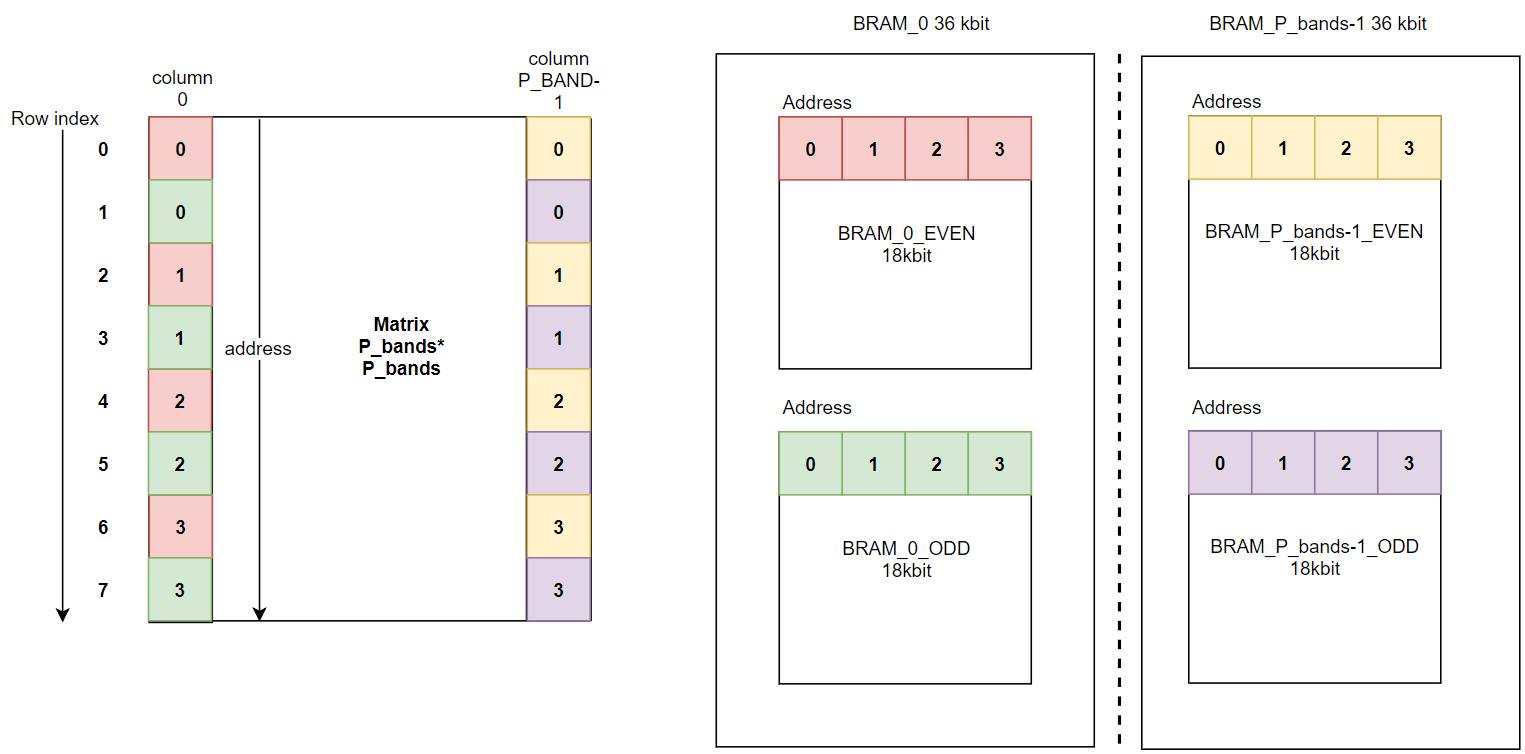
\includegraphics[scale=0.5]{images/bram_addressing_matrix.PNG}
  \caption{Storing matrix elements in different 36kbit BRAMs, storing one column of a matrix per BRAM. Each 36 kbit BRAM consists of two 18kbit BRAM blocks, one block storing even indexes of the matrix column, and one block storing odd indexes of the matrix column.    } 
  \label{fig:BRAM_matrix}
\end{figure}





\section{Inverse computation}
\label{sec:inverse_computation_hw}
Due to its low complexity, the Gauss-Jordan elimination was chosen to compute the inverse. A drawback with this algorithm is that it uses division. Division is an operation that is computationally intensive in hardware, and requires a large amount of logic to be implemented. An early implementation of the Gauss-Jordan elimination by the author included the use of the division operator "/". This is further described in Section \ref{sec:division_operator}.


%This approach utilized $P\_BANDS$ numbers of divisions, to ensure that one row of the inverse matrix could be computed in one clock cycle. The inner loop operation of forward and backward elimination in Figure \ref{fig:gauss_jordan_pseudocode} for this approach is shown in Figure .  A scaling problem became apparent, as this approach utilized too many LUTs as functions.  This is showed in the results, section \ref{sec:synthesis:luts_and_registers_inverse}. 
%Another approach was made, \textbf{INSERT figures here}..

An approach to implement division by adaptive shifting is described in Section \ref{sec:adaptive_shifting}. 

A third approach for computing division was made. This approach utilizes a large number of LUTs. It is further described in Section \ref{sec:LUT_division}.

%%\begin{figure}[H]
%%\centering
%%   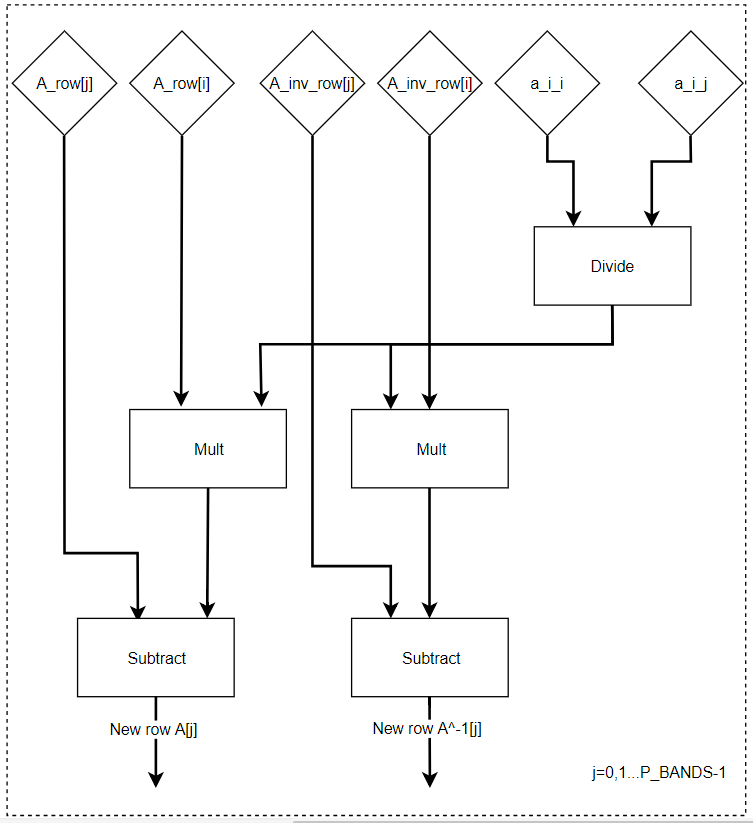
\includegraphics[scale=0.5]{images/inverse_approach_P_BANDS_divisions/inverse_core_old_approach.PNG}
%%  \caption{Architecture showing the first approach to implementing the forward and backward inner loop operation from Figure \ref{fig:gauss_jordan_pseudocode}. $P\_BANDS$ modules marked by the dotted border was synthesized.  } 
%%  \label{fig:inverse_P_BANDS_number_of_divisions}
%%\end{figure}


\subsection{Top level architecture}
The top level architecture of the inverse module can be seen in Figure \ref{fig:top_level_inverse}. This is an implementation of the Gauss-Jordan algorithm shown in Figure \ref{fig:gauss_jordan_pseudocode}. The \textbf{Forward elimination} block correspond to operations marked by the black square in Figure \ref{fig:gauss_jordan_pseudocode}, while \textbf{Backward elimination} and \textbf{Last division} blocks correspond to the operations marked by the red and green squares in Figure \ref{fig:gauss_jordan_pseudocode} respectively, with an exception to the operations shown in Figure \ref{fig:elimination_inner_core_pseudocode}.These operations are part of both the forward elimination and backward elimination blocks in the Gauss-Jordan inverse. They are therefore put in an external process, called \textbf{Elimination core}. 
\\

\textbf{A} and \textbf{A\_inv} are two BRAM36 arrays of size $P\_BANDS$, in which $\textbf{A}$ and $\textbf{A}^{-1}$ are stored, respectively. 

\begin{figure}[H]
\centering
   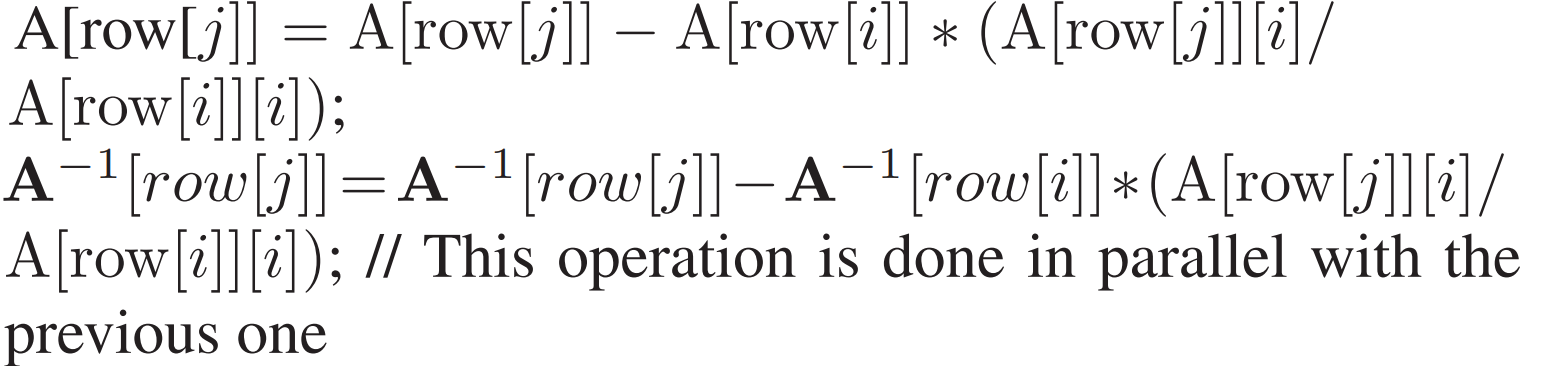
\includegraphics[scale=0.3]{images/inverse_hw/elimination_inner_core_pseudocode.PNG}
  \caption{The operations computed by the \textbf{Elimination core}, utilized by both the \textbf{Forward elimination} and the \textbf{Backward elimination} block.  } 
  \label{fig:elimination_inner_core_pseudocode}
\end{figure}


\begin{figure}[H]
\refstepcounter{figure}
\begin{tabular}{c|c}

   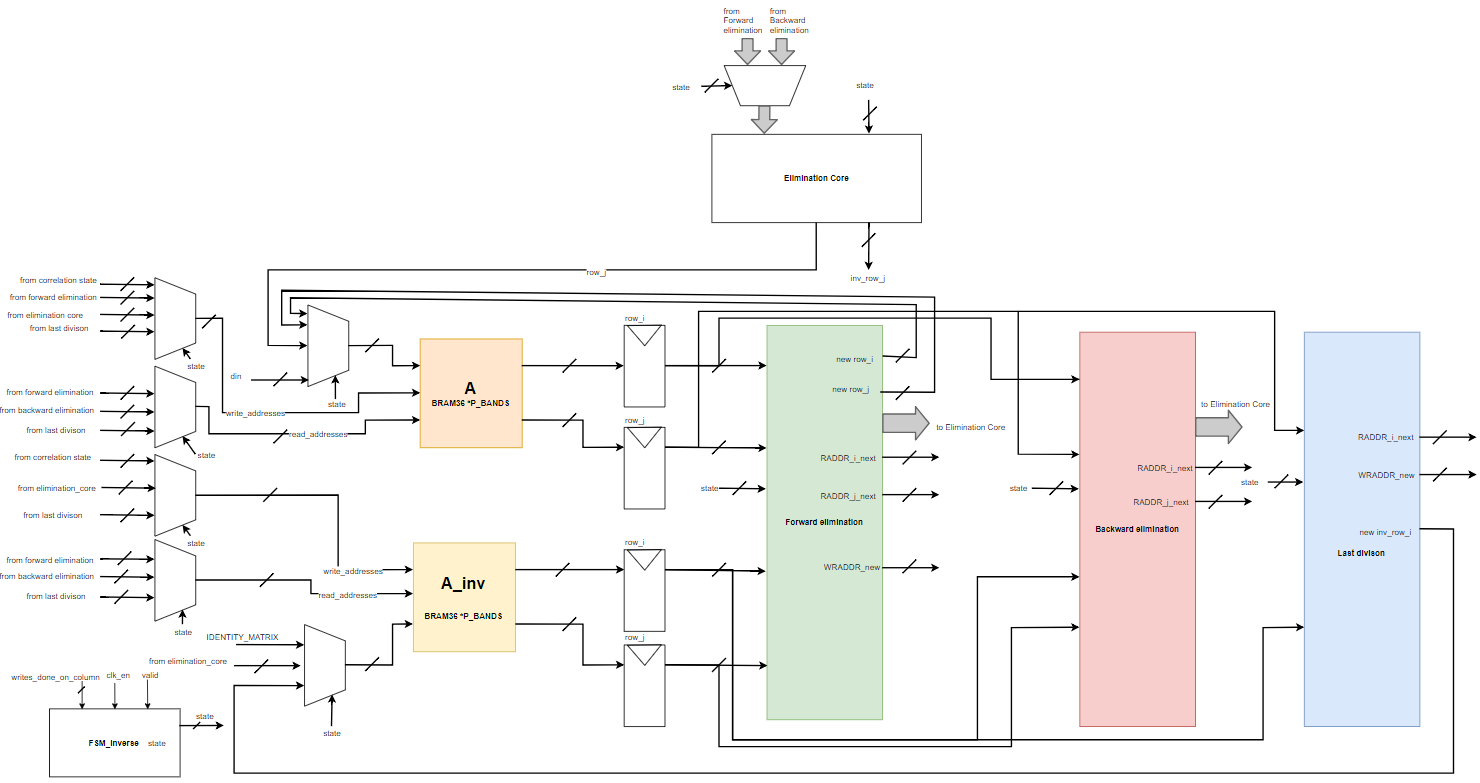
\includegraphics[scale=0.7, angle=90, origin=c]{images/inverse_hw/top_level_architecture_inverse.PNG}
   \rotatebox[origin=c]{90}{ Figure~\thefigure: Top level architecture of the inverse module.}
  %\caption{ \textbf{ROTATE}FSM controlling the architecture shown in Figure  } 
  \end{tabular}
  \label{fig:top_level_inverse}
\end{figure}



\subsection{Top level inverse FSM}
The state machine for the inverse module shown in Figure \ref{fig:top_level_inverse} is shown in Figure \ref{fig:fsm_inverse_matrix}. Its possible states are explained in Table \ref{tab:fsm_inverse}.

\begin{table}[H]
\centering
 \resizebox{1\textwidth}{!}
{\begin{tabular}{l|l}
State                                                                                    & Description                                                                                   \\
\hline
\textbf{Unknown state}                                                                   & An unknown state. The behaviour of the inverse module is unknown. The FSM should transition to state Idle.                                    \\
\textbf{Idle}                                                                            & The inverse module is not performing any operations.                                          \\
\textbf{\begin{tabular}[c]{@{}l@{}}Store\_correlation\_matrix\_\\ in\_BRAM\end{tabular}} & Writing data from correlation module to BRAMs. Two rows written to BRAMs per clock cycle.     \\
\textbf{Forward\_elimination}                                                            & Computing the forward elimination of the Gauss-Jordan elimination as shown in Figure \ref{fig:gauss_jordan_pseudocode}.        \\
\textbf{Backward\_elimination}                                                           & Computing the backward elimination of the Gauss-Jordan elimination as shown in Figure \ref{fig:gauss_jordan_pseudocode}.       \\
\textbf{Last\_division}                                                                  & Computing the last division of the Gauss-Jordan elimination as shown in Figure \ref{fig:gauss_jordan_pseudocode}.              \\
\textbf{Output\_inverse\_matrix}                                                         & Outputting the finished inverse matrix for the pixel. Two rows are outputted per clock cycle.
\end{tabular}}
\caption{States of the inverse FSM}
\label{tab:fsm_inverse}

\end{table}

\begin{figure}[H]
\centering
   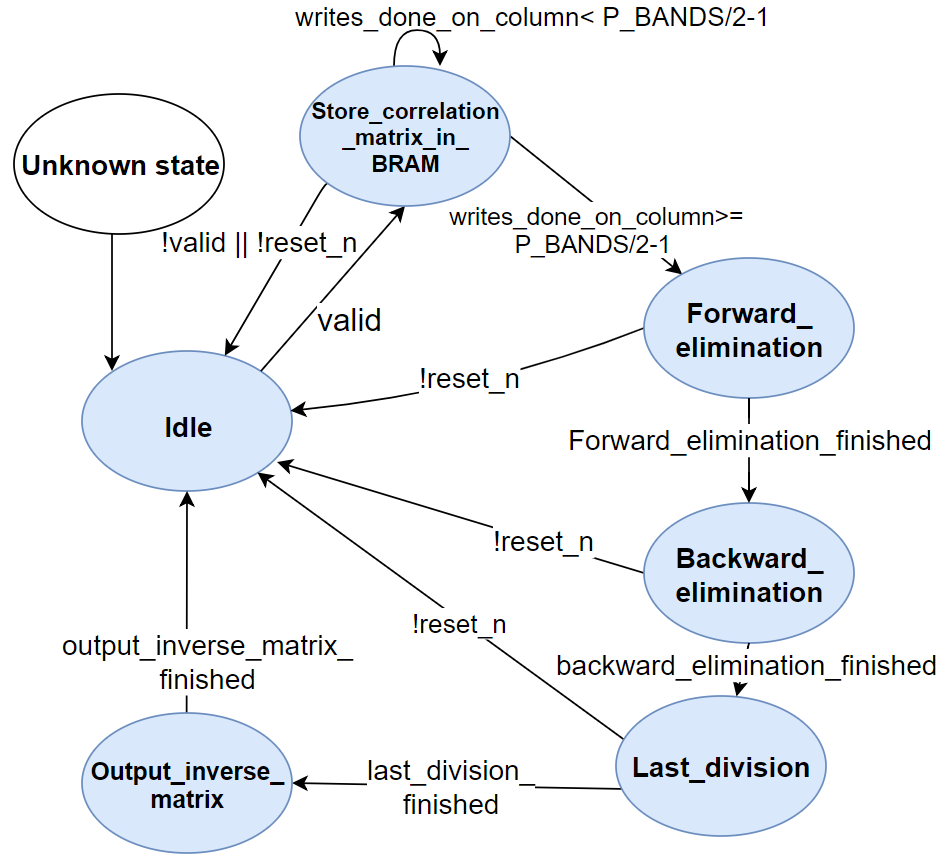
\includegraphics[scale=0.5]{images/inverse_hw/fsm_inverse_matrix.PNG}
  \caption{FSM controlling the architecture shown in Figure \ref{fig:top_level_inverse}.  } 
  \label{fig:fsm_inverse_matrix}
\end{figure}

The inverse module is controlled by the FSM shown in Figure \ref{fig:fsm_inverse_matrix}. 

\subsection{Forward elimination}
Forward elimination is defined as the operations trailing the   of the Gauss-Jordan elimination shown in Figure \ref{fig:gauss_jordan_pseudocode}.


\begin{table}[H]
\centering
 \resizebox{1\textwidth}{!}
{\begin{tabular}{l|l}
State                                                                                    & Description                                                                                   \\
\hline
\textbf{Unknown state}                                                                   & An unknown state. The behaviour of the inverse module is unknown. The FSM should transition to state Idle.                                    \\
\textbf{Idle}                                                                            & The forward elimination module is not performing any operations.                                          \\
\textbf{Check\_diagonal\_element\_is\_zero} & Checking if element row\_i[index\_i]= 0 as done in Gauss-Jordan elimination shown in Figure \ref{fig:gauss_jordan_pseudocode}.     \\
\textbf{Swap\_rows}                                                            & Swapping row\_i and row\_j of the matrix A as described in Figure \ref{fig:gauss_jordan_pseudocode}.        \\
\textbf{Even\_j\_write}                                                           & Updating an even indexed row of the matrix A and $A^{-1}$(described in Figure \ref{fig:gauss_jordan_pseudocode}).       \\
\textbf{Odd\_j\_write}                                                                  & Updating an odd indexed row of the matrix A and $A^{-1}$(described in Figure \ref{fig:gauss_jordan_pseudocode}).   
\end{tabular}}
\caption{States of the forward elimination FSM}
\label{tab:fsm_forward_elimination}

\end{table}


\begin{figure}[H]
\centering
   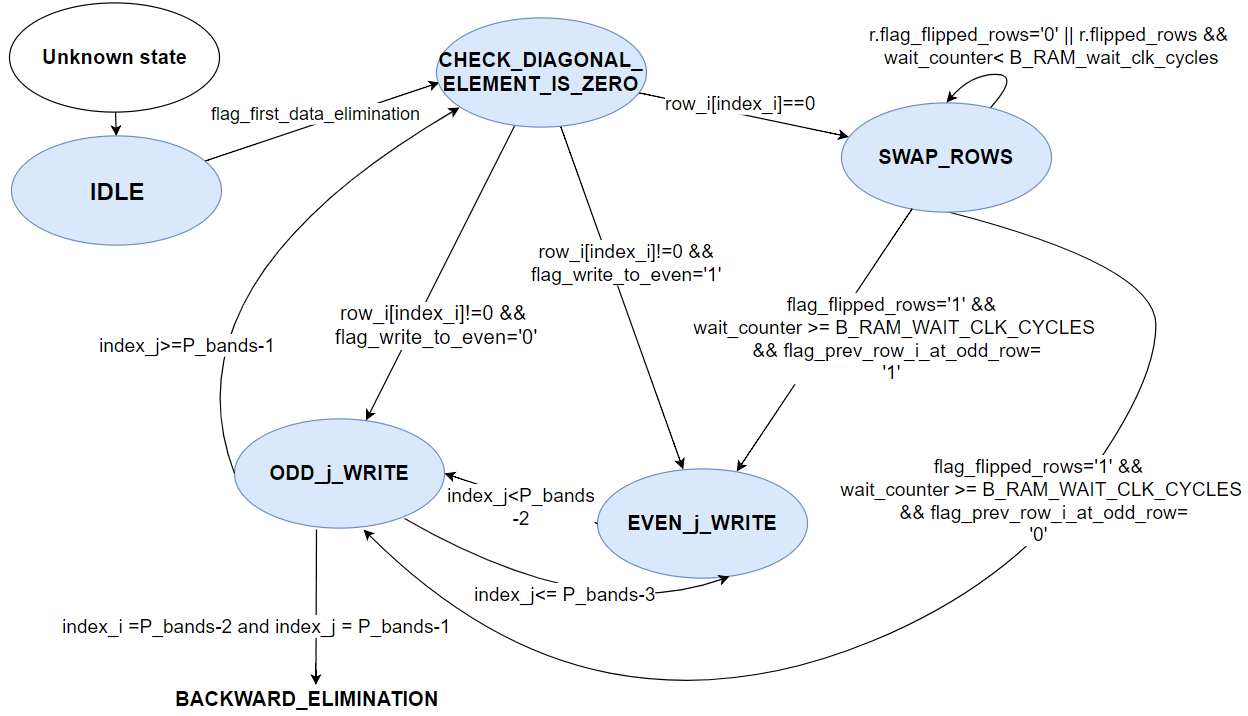
\includegraphics[scale=0.4]{images/inverse_hw/fsm_forward_elimination.png}
  \caption{FSM controlling the forward elimination state shown in Figure \ref{fig:fsm_inverse_matrix}.  } 
  \label{fig:fsm_forward_elimination}
\end{figure}


\subsection{Backward elimination}

\begin{table}[H]
\centering
 \resizebox{1\textwidth}{!}
{\begin{tabular}{l|l}
State                                                                                    & Description                                                                                   \\
\hline
\textbf{Unknown state}                                                                   & An unknown state. The behaviour of the inverse module is unknown. The FSM should transition to state Idle.                                    \\
\textbf{Idle}                                                                            & The forward elimination module is not performing any operations.                                          \\
\textbf{First\_elimination} & Checking if element row\_i[index\_i]= 0 as done in Gauss-Jordan elimination shown in Figure \ref{fig:gauss_jordan_pseudocode}.     \\
\textbf{Odd\_i\_start}                                                            & Starting at a new iteration of the outermost loop of the backward elimination loop in the Gauss-Jordan elimination shown in  \ref{fig:gauss_jordan_pseudocode}. 
\\
&
Starting at an odd row-index of the matrix. Computing A[row\_j] and $A^{-1}$[row\_j], which is at an even index. Updating matrices.       \\

\textbf{Even\_i\_start}                                                            & Starting at a new iteration of the outermost loop of the backward elimination loop in the Gauss-Jordan elimination shown in  \ref{fig:gauss_jordan_pseudocode}.
\\&
Starting at an even row-index of the matrix. Computing A[row\_j] and $A^{-1}$[row\_j], which is at an odd index. Updating matrix.        \\

\textbf{Even\_j\_write}                                                           & Updating an even indexed row of the matrix A and $A^{-1}$(described in Figure \ref{fig:gauss_jordan_pseudocode}).       \\
\textbf{Odd\_j\_write}                                                                  & Updating an odd indexed row of the matrix A and $A^{-1}$(described in Figure \ref{fig:gauss_jordan_pseudocode}).   
\end{tabular}}
\caption{States of the forward elimination FSM}
\label{tab:fsm_forward_elimination}

\end{table}

\begin{figure}[H]
\centering
   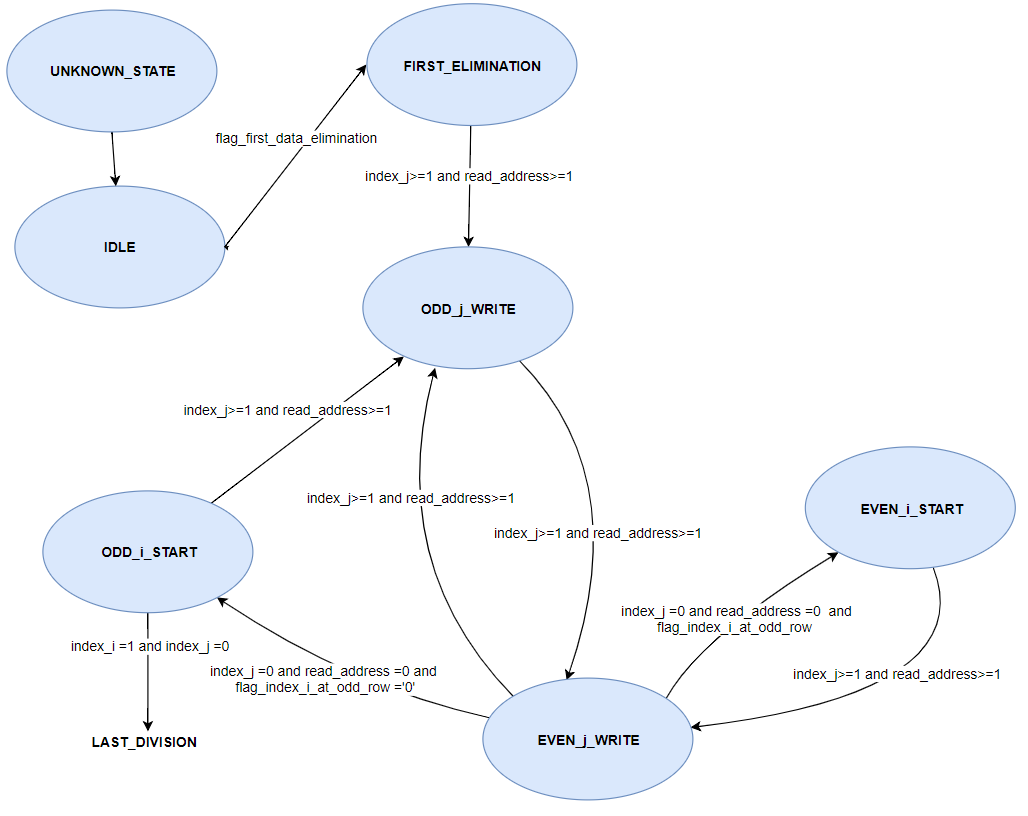
\includegraphics[scale=0.5]{images/inverse_hw/fsm_backward_elimination.PNG}
  \caption{FSM controlling the backward elimination state shown in Figure \ref{fig:fsm_inverse_matrix}.  } 
  \label{fig:fsm_backward_elimination}
\end{figure}

\subsection{Last division}

\begin{table}[H]
\centering
 \resizebox{1\textwidth}{!}
{\begin{tabular}{l|l}
State                                                                                    & Description                                                                                   \\
\hline
\textbf{Unknown state}                                                                   & An unknown state. The behaviour of the inverse module is unknown. The FSM should transition to state Idle.                                    \\
\textbf{Idle}                                                                            & The forward elimination module is not performing any operations.                                          \\


\textbf{Even\_i\_write}                                                           & Updating an even indexed row of the matrix $A^{-1}$(described in Figure \ref{fig:gauss_jordan_pseudocode}).       \\
\textbf{Odd\_i\_write}                                                                  & Updating an odd indexed row of the matrix $A^{-1}$(described in Figure \ref{fig:gauss_jordan_pseudocode}).   
\end{tabular}}
\caption{States of the last division FSM}
\label{tab:fsm_last_division}

\end{table}


\begin{figure}[H]
\centering
   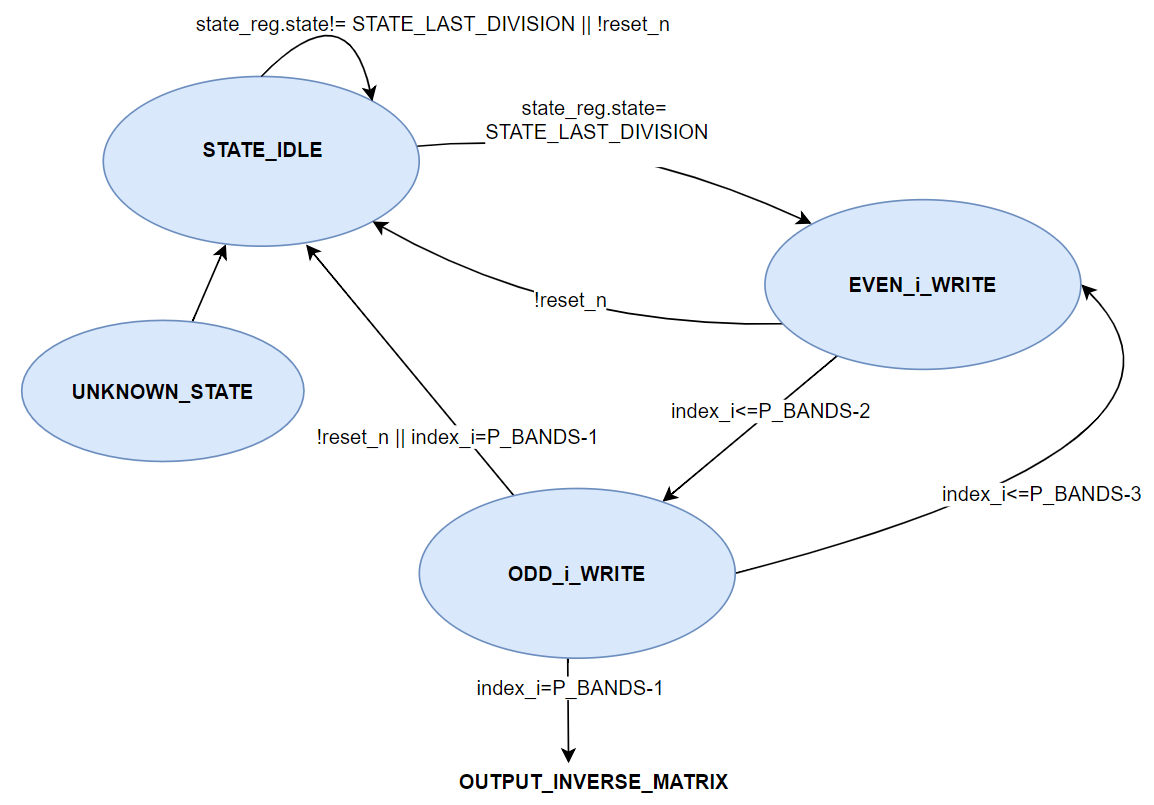
\includegraphics[scale=0.5]{images/inverse_hw/fsm_last_division.PNG}
  \caption{FSM controlling the last\_division state shown in Figure \ref{fig:fsm_inverse_matrix}.  } 
  \label{fig:fsm_last_division}
\end{figure}

\subsection{Memory hierarchy}
The Gauss Jordan inverse requires two matrices to be stored in memory, the matrix $\textbf{A}$ and $\textbf{A}^{-1}$ as shown in Figure \ref{fig:gauss_jordan_pseudocode}. Both of these matrices will be of the same size as the correlation matrix, described in section \ref{sec:mem_management_correlation_matrix}. It is therefore not desirable to store these matrices in registers, but rather in BRAM. By having the same memory structure as described in section \ref{sec:mem_management_correlation_matrix}, using $P\_BANDS$ BRAM 36kbit blocks for each of the matrices, this will enable two rows of each matrix to be written and read per clock cycle. 

\subsection{Inverse pipeline stages}
The inverse module is pipelined into four stages in order to achieve high throughput. The pipeline can be seen in Figure \ref{fig:pipeline_inverse_part_1}, \ref{fig:pipeline_inverse_part_2} and \ref{fig:pipeline_inverse_part_3}.

\begin{figure}[H]
\centering
   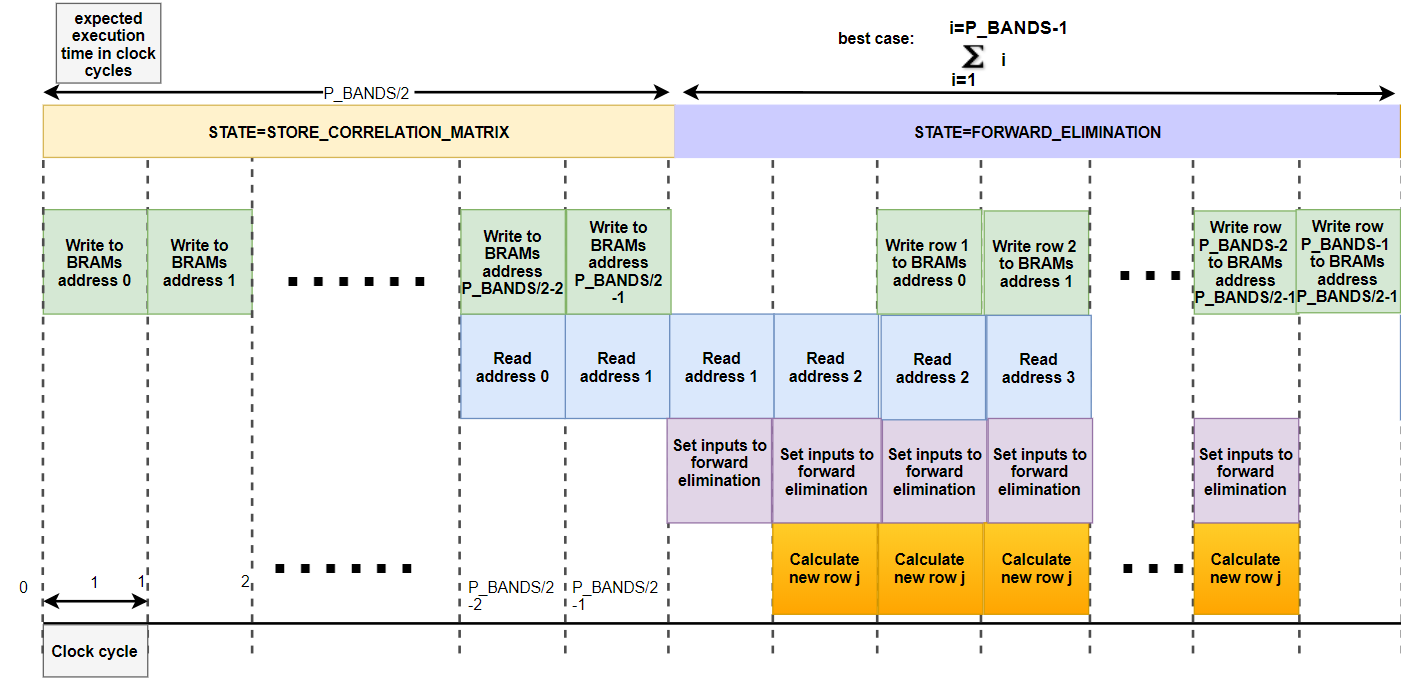
\includegraphics[scale=0.5]{images/estimation_execution_time/pipeline_inverse_matrix_part_1.PNG}
  \caption{Showing pipeline operations in the Store\_correlation\_matrix and Forward\_elimination states.  } 
  \label{fig:pipeline_inverse_part_1}
\end{figure}

\begin{figure}[H]
\centering
   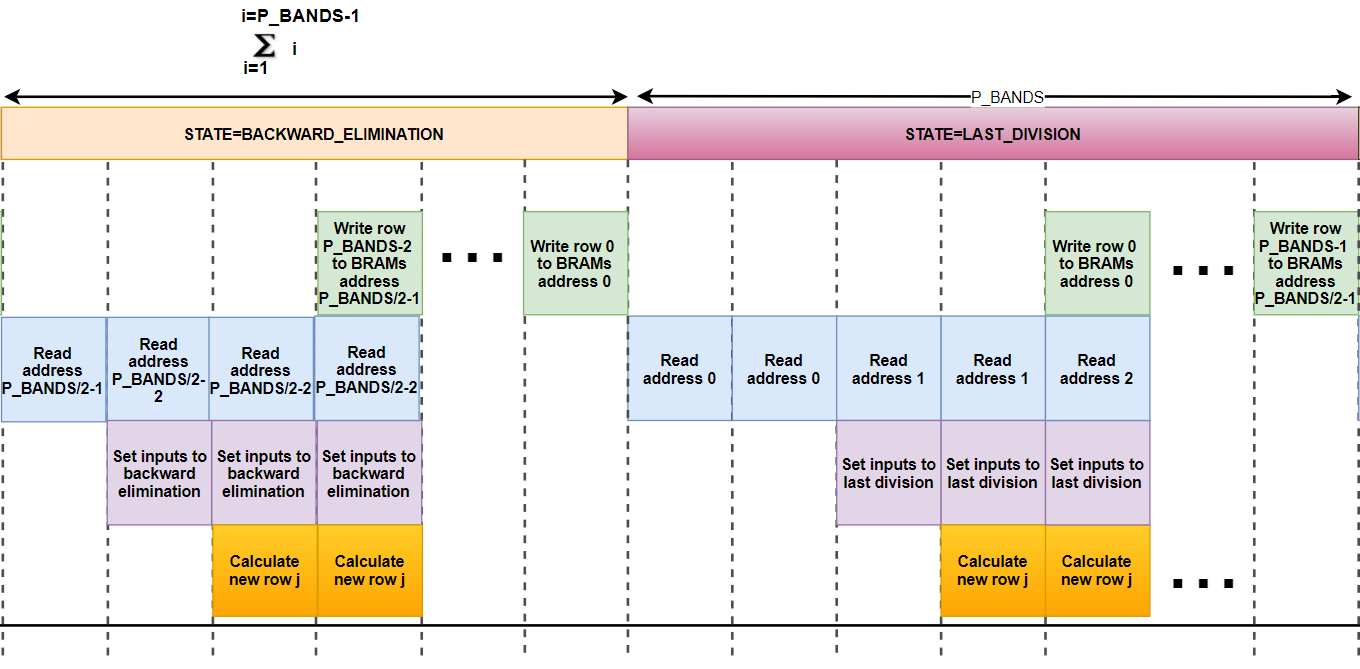
\includegraphics[scale=0.5]{images/estimation_execution_time/pipeline_inverse_matrix_part_2.PNG}
  \caption{Showing pipeline operations in the Forward\_elimination and Last\_division states.  } 
  \label{fig:pipeline_inverse_part_2}
\end{figure}

\begin{figure}[H]
\centering
   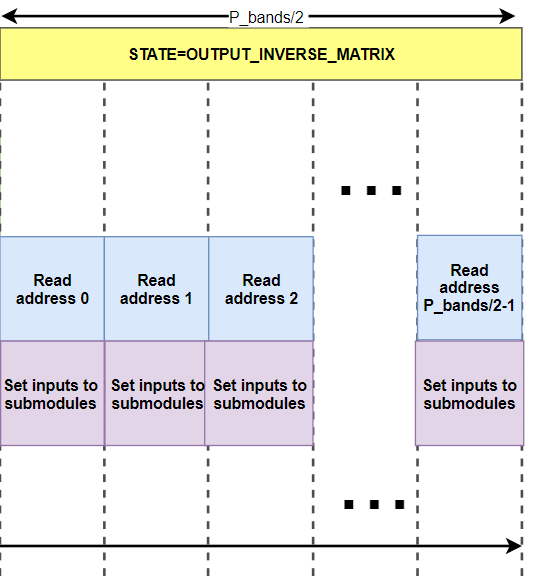
\includegraphics[scale=0.5]{images/estimation_execution_time/pipeline_inverse_matrix_part_3.PNG}
  \caption{Showing pipeline operations in the $Output\_inverse\_matrix$ state.  } 
  \label{fig:pipeline_inverse_part_3}
\end{figure}



\subsection{Execution time expectations}
Using $P\_BANDS$ BRAMs enables to read and write a maximum of two rows of each of the matrices $\textbf{A}$ and $\textbf{A}^{-1}$ per clock cycle.  Assuming that each of the row-operations in the Gauss-Jordan elimination can be calculated within one clock cycle, it is possible to do an estimation of the expected execution time in clock cycles for the inverse computation per pixel. \\

Expected execution time for the different states is shown in Figure \ref{fig:pipeline_inverse_part_1}, \ref{fig:pipeline_inverse_part_2} and \ref{fig:pipeline_inverse_part_3}. For state $Forward\_elimination$, the execution time will be greater if it is necessary to swap rows, shown by the state $SWAP\_ROWS$ in Figure \ref{fig:fsm_forward_elimination}. The worst case execution time of $Forward\_elimination$ is assumed to be when the first element of the matrix $\textbf{A}$ has a zero element at row(i,i) and all other rows,except the last row, has a zero element at row(j,j). \\

A worst case and a best case execution time, $inv\_worst\_case$ and $inv\_best\_case$, for the computation of the inverse per pixel is then estimated. The estimations are shown in Equation \ref{eq:inv_worst_case} and \ref{eq:inv_best_case}.$N\_STATES\_INV$ is the number of valid states in the inverse top level module, shown in Figure \ref{fig:fsm_inverse_matrix}. $worst\_case\_ex\_state$ is the set of expected worst case execution times for the states.  $best\_case\_ex\_state$ is the set of expected best case execution times for the states. 

\begin{equation}
\begin{split}
inv\_worst\_case & = \sum_{i=0}^{N\_STATES\_INV}worst\_case\_ex\_state(i) \\
& =\underbrace{\frac{P\_BANDS}{2} }_\text{STORE\_CORRELATION\_MATRIX}  + \overbrace{\sum_{i=0}^{P\_BANDS-1}i + P\_BANDS}^\text{STATE\_FORWARD\_ELIMINATION} \\
& + \underbrace{\sum_{i=0}^{P\_BANDS-1}i}_\text{STATE\_BACKWARD\_ELIMINATION}  
 +
\overbrace{P\_BANDS}^\text{LAST\_DIVISION} + \underbrace{P\_BANDS/2}_\text{OUTPUT\_INVERSE\_MATRIX}\\
& = 3P\_BANDS + 2\sum_{i=0}^{P\_BANDS-1}i
\end{split}
\label{eq:inv_worst_case}
\end{equation}


\begin{equation}
\begin{split}
inv\_best\_case & = \sum_{i=0}^{N\_STATES\_INV}best\_case\_ex\_state(i) \\
& = \underbrace{\frac{P\_BANDS}{2} }_\text{STORE\_CORRELATION\_MATRIX}  + \overbrace{\sum_{i=0}^{P\_BANDS-1}i }^\text{STATE\_FORWARD\_ELIMINATION} \\
& + \underbrace{\sum_{i=0}^{P\_BANDS-1}i}_\text{STATE\_BACKWARD\_ELIMINATION}  
 +
\overbrace{P\_BANDS}^\text{LAST\_DIVISION} + \underbrace{P\_BANDS/2}_\text{OUTPUT\_INVERSE\_MATRIX}\\
& = 2P\_BANDS + 2\sum_{i=0}^{P\_BANDS-1}i
\end{split}
\label{eq:inv_best_case}
\end{equation}

Figure \ref{fig:estimated_time_inverse} shows the estimated execution time in seconds for computing the inverse for all pixels in the hyperspectral image, for an image size of 1088x576. 

\begin{figure}[H]
\hbox{\hspace*{-3cm}                                                           

   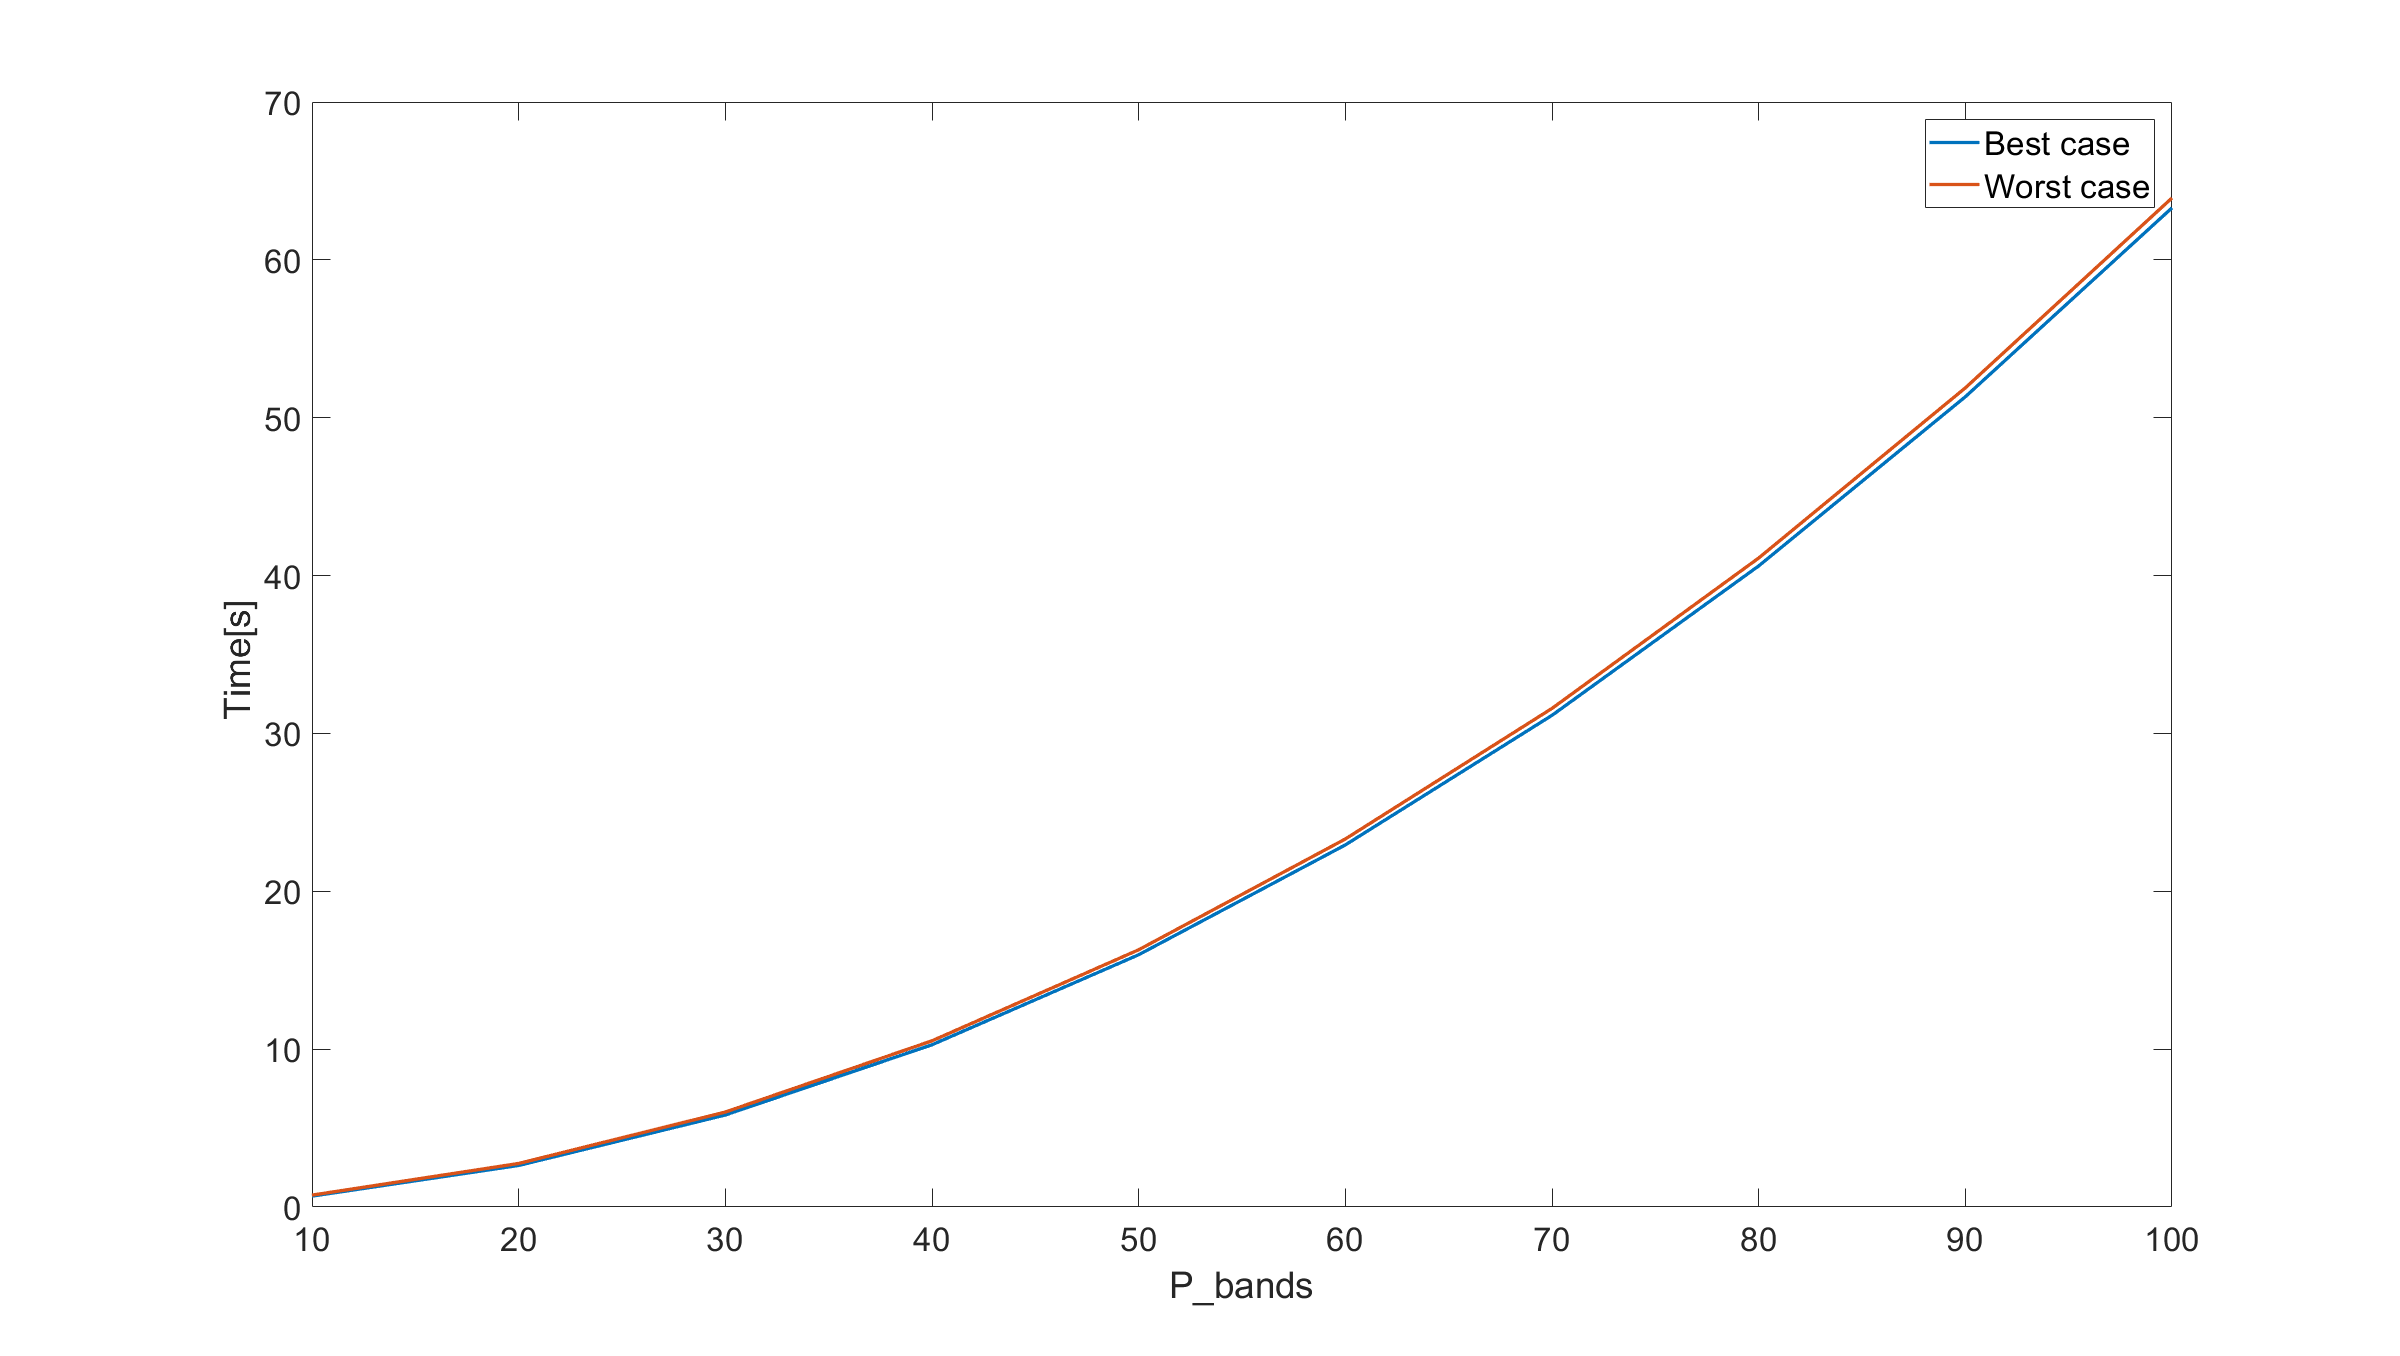
\includegraphics[scale=0.4]{images/estimated_execution_time_inverse_computation_in_seconds.png}}
  \caption{Estimated execution time for inverse matrix computation for an image of 1088x576, in seconds. The horizontal line marks the 54 second processing specification set by the SmallSat project.  } 
  \label{fig:estimated_time_inverse}
\end{figure}
%%\subsubsection{Inverse computation}
%%Estimated execution time backward elimination:
%%\begin{equation}
%%    B=\sum_{i=1}^{i=P_{BANDS}-1} i
%%\end{equation}

\subsection{Division}
\label{sec:division_implementation}
This section describes the implementation of division used in the Gauss-Jordan elimination.  The semantics used to described the division operation will be $C=B*\frac{1}{A}$ where $C,B$ and $A $ are integer variables. This corresponds to the inner loop operation for Last division shown in Figure \ref{fig:gauss_jordan_pseudocode}.


\subsubsection{Using division operator "/"}
\label{sec:division_operator}



%%\begin{figure}[H]
%%\centering
%%   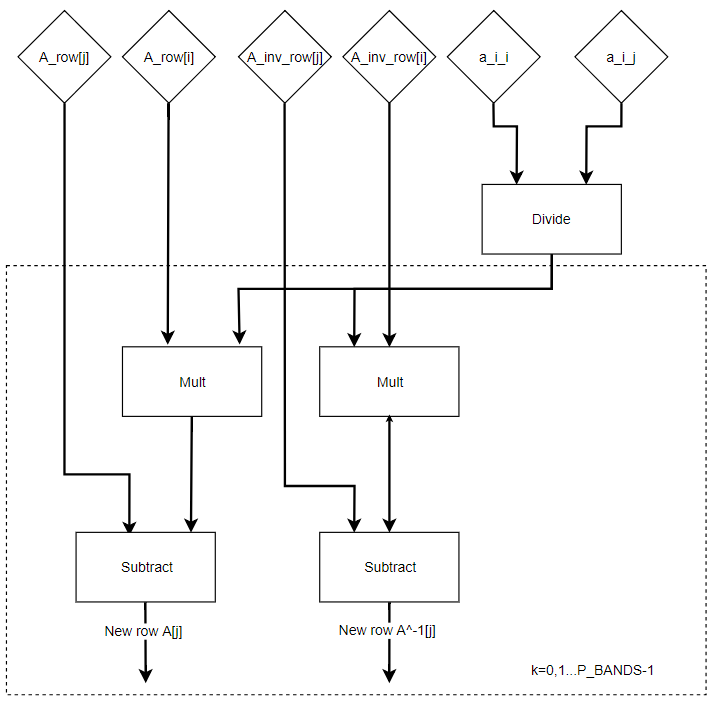
\includegraphics[scale=0.5]{images/inverse_hw/inverse_core_division_approach.PNG}
%%  \caption{Architecture of the \textbf{Elimination core} in Figure \ref{fig:top_level_inverse}, using division operator "/" for integer datatype in VHDL. $k$= $P\_BANDS$ modules marked by the dotted square is implemented in order to compute one row per clock cycle.  } 
%%  \label{fig:adaptive_shifting}
%%\end{figure}

To evaluate if division could be implemented by using the "/" operator, the $\textbf{Last division}$ block was synthesized, and the critical path evaluated, to see if the timing specification of 100 MHz operating frequency could be met. Results for different divisor -and-divident bit width is presented in Table \ref{tab:division_operator_logic_delays}. 


\begin{table}[H]
    \centering
    \begin{tabular}{c|c|c}
    \textbf{Bit width divisor and dividend} &\textbf{Logic delay[ns]}&\textbf{Max frequency[MHz] } \\
         32&72.498 &13.79 \\
         13 &19.726 &50.69\\
         10 & 16.032&62.37 \\
         8 & 12.74&78.49 \\
         6&9.530& 104.93\\
         
    \end{tabular}
    \caption{Synthesis results for ZedBoard Zynq Evaluation and Development Kit Z7020 for \textbf{Last division} shown in Figure \ref{fig:top_level_inverse}, implementing the product $C= B*\frac{1}{A}$. Bit width for factor $B$ is 32 bit.}
    \label{tab:division_operator_logic_delays}
\end{table}{}
%% Insert table here, with widths and delays

\subsubsection{Adaptive shifting}
\label{sec:adaptive_shifting}
        To avoid using the division operator the adaptive shifting approach shown in \ref{fig:adaptive_shifting} has been implemented. It approximates the divisor by an adaptive number of shift operations, as the divisor is not constant. To achieve this, the most significant bit(MSB) of the divisor is first checked to evaluate if the divisor is a negative number. If it is, the divisor is negated. The block \textbf{Find MSB} finds the MSB of the unsigned divisor. In parallel with this, $PIXEL\_DATA\_WIDTH*2-1$ numbers of shift operation processes shifts the unsigned divisor by $n\_shifts$=[1,2...$PIXEL\_DATA\_WIDTH*2-1$]. The remainders after shifting is sent to the \textbf{Choose best approximation} block. This block choose the best approximation depending upon the index of the MSB and the remainders after shifting. The best approximation to the divisor will be a shift operation by MSB or MSB+1 number of shifts. Each element of the row is then shifted in parallel to compute the approximate division in one clock cycle. If the divisor is a negative number, the row is negated before outputting data to register.
        \\
        The design shown in Figure \ref{fig:adaptive_shifting} was synthesized for Zedboard Zynq Evaluation and Development kit Z7020 to check timing. The max logic delay was $6.932$ns which gives a max operating frequency of 144.25 MHz, not accounting for net delay. 


The adaptive shifting will have an error of \textbf{FIND largest error.}. 

%\textbf{Mention the fact that r\_i\_i\_half is added before dividing. This is because of integer rounding in hardware/vivado}


\begin{figure}[H]
\centering
   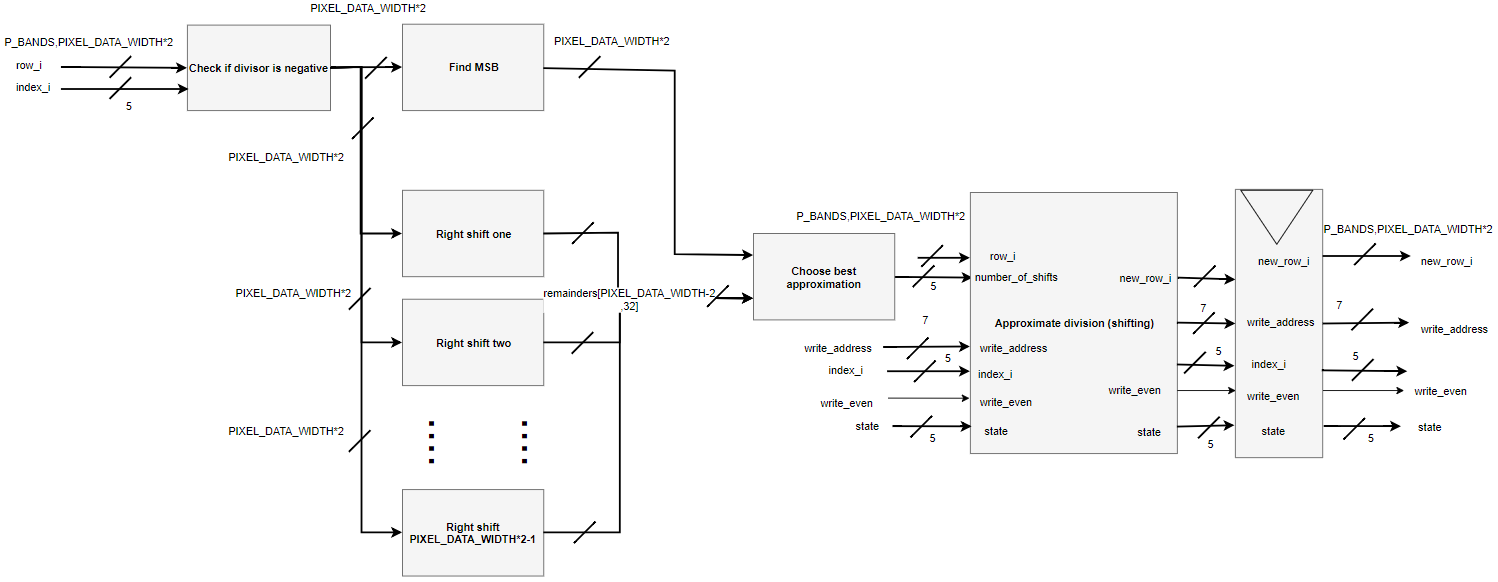
\includegraphics[scale=0.5]{images/approximate_division/last_division.PNG}
  \caption{Architecture of block \textbf{Last division}, approaching division with an adaptive number of shifts.   } 
  \label{fig:adaptive_shifting}
\end{figure}


\subsubsection{LUT approach}
\label{sec:LUT_division}
Instead of computing the division in the operation $C= B*\frac{1}{A}$, an approach based on the solution in \cite{cite:how_to_implement_division} was made. The approach utilizes LUTs to store the array $divisor\_inv$=$\frac{2^{DIV\_PRECISION}}{A}$, where $A=1,2...2^{DIV\_PRECISION}$ and $DIV\_PRECISION$ is the bit width of the divisor and the dividend. Instead of dividing by an integer $A$, $A$ is used as an index to look up in LUTs(number of LUTs depending upon $DIV\_PRECISION$) storing the $divisor\_inv$. $divisor\_inv(A)$ is then multiplied by $B$, which yields product $C$. $C$ is then right shifted $DIV\_PRECISION$ spaces. This can be seen in Equation \ref{LUT_operations}.

\begin{equation} \label{LUT_operations}
\begin{split}
C= shift\_right(B*\frac{2^{DIV\_PRECISION}}{A},DIV\_PRECISION)
\end{split}
\end{equation}

The code for inferring the LUTs for storage of $divisor\_inv$ is shown in Listing \ref{lst:lut_division}, examplified for DIV\_PRECISION=4.  

\lstinputlisting[caption={LUT division approach examplified for DIV\_PRECISION = 4.},label={lst:lut_division},style=customc]{code/lut_4_bit_example.vhd}

The architecture of the \textbf{Last division} block, utilizing this LUT approach, is shown in figure \ref{fig:top_last_division_lut_approach}. If choosing $DIV\_PRECISION$< $PIXEL\_DATA\_WIDTH*2$, an adaptive shifting approach is utilized. 
\\

\begin{figure}[H]
\hbox{\hspace*{-2cm}                                                           

   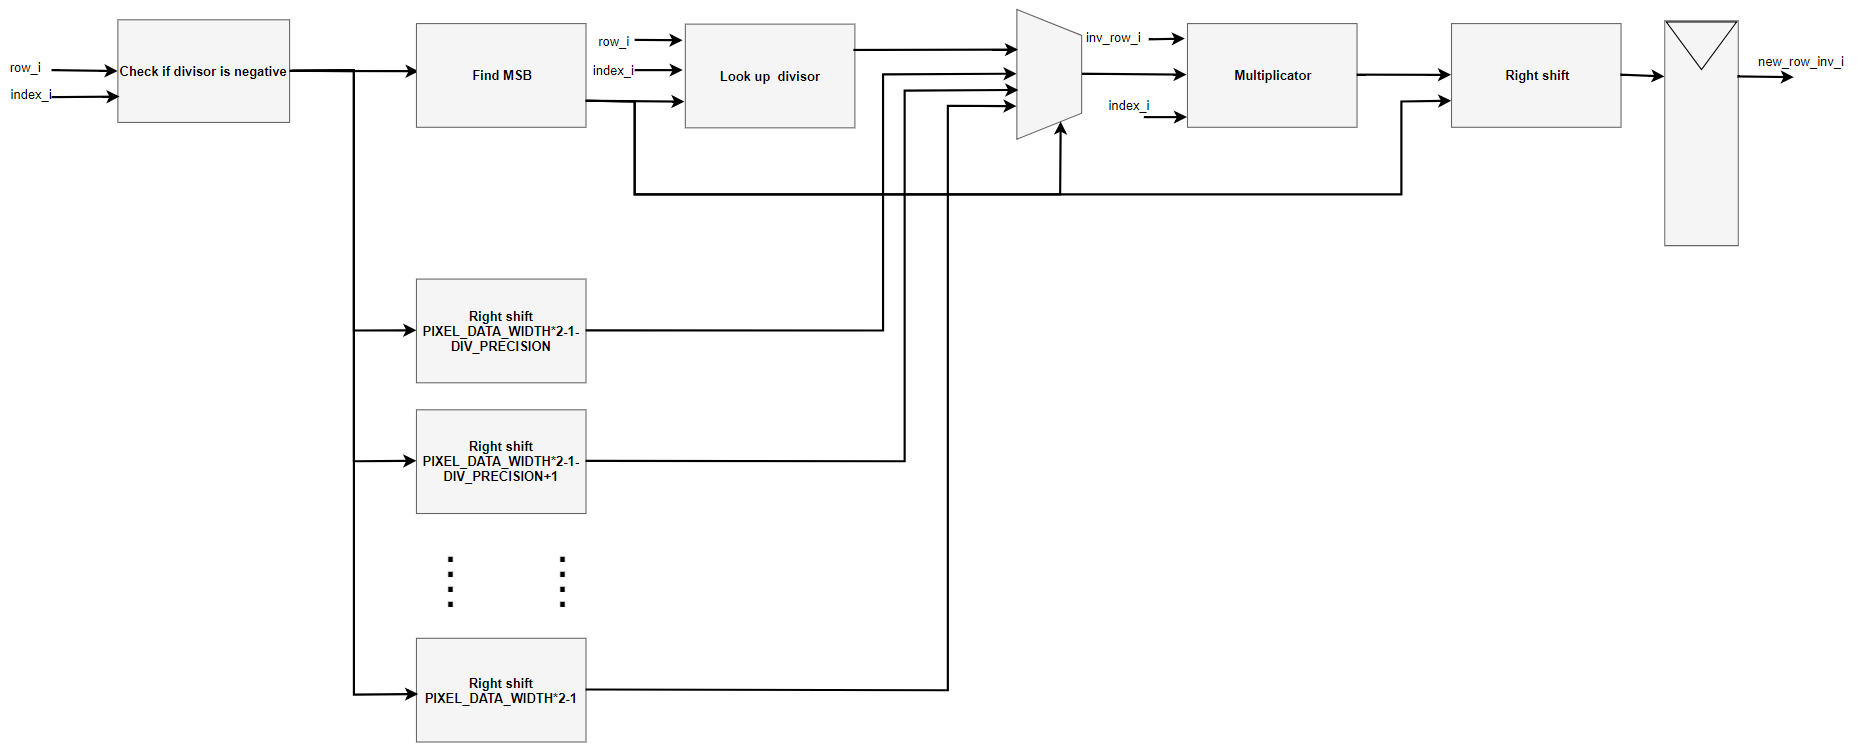
\includegraphics[scale=0.45]{images/approximate_division/top_last_division_lut_approach_dataflow.PNG}}
  \caption{Architecture of block \textbf{Last division}, computing division using the LUT approach.   } 
  \label{fig:top_last_division_lut_approach}
\end{figure}